%
%===================================================================================================
%
\documentclass[aspectratio=169]{beamer}
%
%===================================================================================================
%
%
%===================================================================================================
%
% Main Modular Preamble Loader
%
%===================================================================================================

%
%===================================================================================================
%
% Packages
%
%===================================================================================================

\usepackage[absolute,overlay]{textpos}

\usepackage[utf8]{inputenc}
\usepackage[T1]{fontenc}

\usepackage{amsmath}
\usepackage{amsfonts}
\usepackage{amssymb}
% the following order matter!!!
\usepackage{lmodern}
\usepackage{bm}

\usepackage{array}
\usepackage{booktabs}
\usepackage{colortbl}
\usepackage{multirow}

\usepackage{graphicx}
\usepackage{tikz}
\usepackage{pgfplots}

\usepackage{framed}
\usepackage{empheq}

\usepackage{xcolor}
\usepackage{soul}

\usepackage{hyperref}
\usepackage{pgfpages}

%\usepackage{minted}

\usepackage[most]{tcolorbox}
\tcbuselibrary{listings}

\pgfplotsset{compat=1.14}
%
%===================================================================================================
%
% TikZ Libraries
%
%===================================================================================================

\usetikzlibrary{
    arrows.meta,
    positioning,
    fit,
    calc,
    shapes.geometric,
    backgrounds,
    matrix
}

% ── Reusable TikZ styles ─────────────────────────────────────
\tikzset{
  block/.style   = {draw, rounded corners, minimum width=2.0cm,
                    minimum height=0.60cm, align=center, font=\small},
  sblock/.style  = {draw, rounded corners, minimum width=1.4cm,
                    minimum height=0.55cm, align=center, font=\small},
  token/.style   = {draw, rounded corners, minimum width=1.1cm,
                    minimum height=0.55cm, font=\small},
  arr/.style     = {->, thick, boIndigo},
  arrg/.style    = {->, gray!60, line width=0.7pt}
}

%
%===================================================================================================
%
% Custom Colors
%
%===================================================================================================

% General accents
\definecolor{accent}{RGB}{200,60,50}
\definecolor{Accent}{RGB}{240,170,0}
\definecolor{accentblue}{HTML}{457B9D}
\definecolor{accentred}{HTML}{E63946}

% Course colors
\definecolor{CourseBlue}{RGB}{47,53,163}
\definecolor{unibo}{RGB}{0,68,136}
\definecolor{uniboblue}{RGB}{0,54,132}
\definecolor{uniblue}{RGB}{0,76,147}
\definecolor{unired}{RGB}{155,0,20}
\definecolor{codebg}{RGB}{248,248,248}
\definecolor{lightblue}{RGB}{220,235,250}

% Code colors
\definecolor{codebg}{rgb}{0.97,0.97,0.97}
\definecolor{codeborder}{rgb}{0.8,0.8,0.8}

% Neural-network / layer colors
\definecolor{w1col}{RGB}{255,180,0}
\definecolor{w2col}{RGB}{180,90,30}
\definecolor{b1col}{RGB}{0,255,0}
\definecolor{layer1violet}{HTML}{800080}
\definecolor{layer2red}{HTML}{FF0000}
\definecolor{updategreen}{HTML}{228B22}

% Financial colors
\definecolor{finblue}{RGB}{0,51,102}
\definecolor{fingray}{RGB}{100,100,100}
\definecolor{fingreen}{RGB}{0,100,0}
\definecolor{finred}{RGB}{178,34,34}

% Semantic colors
\definecolor{darkgreen}{RGB}{0,120,60}
\definecolor{DeepRed}{RGB}{180,45,45}
\definecolor{Forest}{RGB}{34,120,70}

% Light background colors
\definecolor{lightblue}{RGB}{210,230,250}
\definecolor{lightgreen}{RGB}{210,245,210}
\definecolor{lightorange}{RGB}{255,235,205}
\definecolor{lightred}{RGB}{255,220,220}
\definecolor{lightyellow}{RGB}{255,255,210}

% Soft background colors
\definecolor{SoftBlue}{RGB}{225,235,255}
\definecolor{SoftGray}{RGB}{245,245,245}
\definecolor{SoftGreen}{RGB}{228,243,232}
\definecolor{SoftOrange}{RGB}{255,244,224}

% Modern palette
\definecolor{navy}{RGB}{15,27,61}
\definecolor{deepblue}{RGB}{22,38,83}
\definecolor{midblue}{RGB}{30,58,110}
\definecolor{teal}{RGB}{13,148,136}
\definecolor{lightgray}{RGB}{148,163,184}
\definecolor{ice}{RGB}{202,220,252}
\definecolor{gold}{RGB}{245,158,11}
\definecolor{coral}{RGB}{249,115,22}
\definecolor{darktext}{RGB}{30,41,59}
\definecolor{offwhite}{RGB}{240,244,250}
\definecolor{boIndigo}{RGB}{55,0,153}

\definecolor{NavyBlue}{RGB}{20,40,100}
\definecolor{SteelBlue}{RGB}{70,130,180}
\definecolor{LightGray}{RGB}{245,245,250}
\definecolor{AccentGold}{RGB}{210,160,30}

\definecolor{futC} {gray}{0.60}
\definecolor{actC} {RGB}{15, 82, 186}
\definecolor{doneC}{RGB}{25, 25,  25}

\definecolor{GateOrange}{RGB}{230,120,0}
\definecolor{GatePurple}{RGB}{110,0,150}
\definecolor{CellGold}{RGB}{160,120,0}

% Alias
\colorlet{bolight}{boIndigo!10}
\colorlet{bodark}{boIndigo!85!black}
\colorlet{actFill}{actC!10}   % light-blue cell background when active


%
%===================================================================================================
%
% Beamer Theme and Style
%
%===================================================================================================

\usetheme{Madrid}
\usecolortheme{default}

%
%===================================================================================================
%
% Beamer Color Customization
%
%===================================================================================================

\setbeamercolor{title}{fg=white,bg=CourseBlue}
\setbeamercolor{frametitle}{fg=white,bg=CourseBlue}
\setbeamercolor{structure}{fg=CourseBlue}

\setbeamercolor{block title}{fg=white,bg=CourseBlue}
\setbeamercolor{block body}{fg=black,bg=SoftGray}

\setbeamercolor{item projected}{fg=white,bg=CourseBlue}

\setbeamercolor{section in head/foot}{fg=white,bg=CourseBlue}
\setbeamercolor{subsection in head/foot}{fg=white,bg=CourseBlue!80!black}
\setbeamercolor{author in head/foot}{fg=white,bg=CourseBlue!90!black}
\setbeamercolor{title in head/foot}{fg=white,bg=CourseBlue!70!black}
\setbeamercolor{date in head/foot}{fg=white,bg=CourseBlue!90!black}

%
%===================================================================================================
%
% Navigation Symbols and Itemize Style
%
%===================================================================================================

\setbeamertemplate{navigation symbols}{}

\setbeamertemplate{itemize item}{\color{CourseBlue}$\blacktriangleright$}
\setbeamertemplate{itemize subitem}{\color{CourseBlue}$\bullet$}
%
%===================================================================================================
%
% Mathematical Macros
%
%===================================================================================================

\newcommand{\vect}[1]{\bm{#1}}
\newcommand{\R}{\mathbb{R}}

\newcommand{\bx}{\bm{x}}
\newcommand{\bh}{\bm{h}}
\newcommand{\bw}{\bm{w}}
\newcommand{\bW}{\bm{W}}
\newcommand{\bb}{\bm{b}}
\newcommand{\diag}{\operatorname{diag}}

\newcommand{\vw}{\mathbf{w}}
\newcommand{\vwt}{\tilde{\mathbf{w}}}
%
%===================================================================================================
%
% Text and Highlighting Macros
%
%===================================================================================================

\newcommand{\soft}[1]{\textcolor{CourseBlue}{\textbf{#1}}}

\newcommand{\highlight}[1]{%
    \colorbox{yellow!25}{$\displaystyle #1$}
}

%
%===================================================================================================
%
% Beamer-Compatible Highlight Fix for the soul Package
%
%===================================================================================================

\makeatletter
\let\HL\hl
\renewcommand\hl{%
  \let\set@color\beamerorig@set@color
  \let\reset@color\beamerorig@reset@color
  \HL}
\makeatother

%
%===================================================================================================
%
% Custom Intuition Box
%
%===================================================================================================

\newcommand{\intuition}[1]{%
  \vspace{4pt}
  \begin{tikzpicture}
    \node[
        fill=offwhite,
        rounded corners=4pt,
        inner sep=6pt,
        text width=0.92\textwidth
    ] {%
      \textcolor{teal}{\textbf{Intuition:}} 
      \textcolor{darktext}{\small #1}
    };
  \end{tikzpicture}
}


\newcommand{\dmodel}{d_{\mathrm{model}}}
\newcommand{\dff}{d_{\mathrm{ff}}}
\newcommand{\dk}{d_k}
\newcommand{\dv}{d_v}

% ─────────────────────────────────────────────────────────────────────
%  \drawcell{cx}{cy}{border-color}{fill-color}
%  Draws the RNN cell rectangle + 3 neuron circles at (cx, cy).
% ─────────────────────────────────────────────────────────────────────
\newcommand{\drawcell}[4]{%
  \fill[#4, rounded corners=3pt]
    ({#1-0.68},{#2-1.10}) rectangle ({#1+0.68},{#2+1.10});
  \draw[color=#3, line width=1.5pt, rounded corners=3pt]
    ({#1-0.68},{#2-1.10}) rectangle ({#1+0.68},{#2+1.10});
  \draw[color=#3, line width=0.9pt] (#1,{#2+0.55}) circle(0.21);
  \draw[color=#3, line width=0.9pt] (#1, #2)        circle(0.21);
  \draw[color=#3, line width=0.9pt] (#1,{#2-0.55}) circle(0.21);
}
% Bold vectors shortcut (match existing notation)
\newcommand{\vct}[1]{\bm{#1}}

%
%===================================================================================================
%
\title[]{Chapter 3 -- Sequential Models and the Road to Attention}
\subtitle{Advanced Machine Learning for Finance}
\author{Giovanni Della Lunga}
\institute{Master's Degree in Quantitative Finance -- University of Bologna}
\date{Bologna -- 2026}
%
%===================================================================================================
%
\AtBeginSection[]{
\begin{frame}
\vfill
\centering
\begin{beamercolorbox}[sep=10pt,center,shadow=true,rounded=true]{title}
\usebeamerfont{title}\insertsectionhead\par
\end{beamercolorbox}
\vfill
\end{frame}
}
%
%===================================================================================================
%
\begin{document}
%
%===================================================================================================
%
\begin{frame}
    \titlepage
\end{frame}
%__________________________________________________________________________
%
\section{Introduction}
%__________________________________________________________________________
%
\begin{frame}{Where We Are in the Course}
\begin{block}{Picking up from Lesson 2}
We built the representation toolkit: from perceptrons to dense word vectors.
Lesson 3 asks how to process \textbf{sequences} of such representations ---
and what architectures are needed before transformers become possible.
\end{block}

\vspace{0.2cm}
\begin{center}
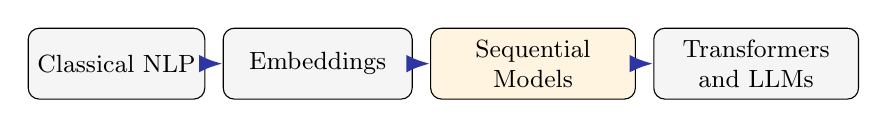
\begin{tikzpicture}[node distance=0.5cm and 0.22cm, every node/.style={font=\small}]
\node[draw,rounded corners,fill=SoftGray, minimum width=2.2cm,minimum height=0.9cm]
    (a) {Classical NLP};
\node[draw,rounded corners,fill=SoftGray, right=of a, minimum width=2.4cm,minimum height=0.9cm]
    (b) {Embeddings};
\node[draw,rounded corners,fill=SoftOrange,right=of b, minimum width=2.6cm,minimum height=0.9cm,align=center]
    (c) {Sequential\\Models};
\node[draw,rounded corners,fill=SoftGray, right=of c, minimum width=2.6cm,minimum height=0.9cm,align=center]
    (d) {Transformers\\and LLMs};
\draw[-{Latex[length=3mm]},very thick,CourseBlue] (a) -- (b);
\draw[-{Latex[length=3mm]},very thick,CourseBlue] (b) -- (c);
\draw[-{Latex[length=3mm]},very thick,CourseBlue] (c) -- (d);
\end{tikzpicture}
\end{center}

\vspace{0.15cm}
\begin{itemize}
    \item Lesson 2: from hard thresholds to dense word representations.
    \item Lesson 3: from fixed vectors to \textbf{architectures that process ordered sequences}.
    \item The endpoint is the encoder-decoder model --- the direct architectural precursor of transformers.
\end{itemize}
\end{frame}
%
%..................................................................
%
\begin{frame}{Learning Objectives of This Lesson}
\small
By the end of the lesson, students should be able to:
\begin{itemize}
    \item identify what makes data sequential and why order matters for NLP;
    \item write the forward-pass equations of a recurrent neural network and explain parameter sharing;
    \item explain backpropagation through time and derive the vanishing gradient argument
          from the spectral norm of a product of Jacobians;
    \item describe how gating mechanisms in GRU and LSTM create near-identity gradient paths;
    \item distinguish the encoder role from the decoder role in a sequence-to-sequence model;
    \item identify the fixed-vector bottleneck as the conceptual pressure that leads to attention.
\end{itemize}

\begin{alertblock}{Guiding question}
How can a neural model read a sentence of arbitrary length and produce a meaningful output ---
possibly of a \emph{different} length --- while retaining long-range dependencies?
\end{alertblock}
\end{frame}
%
%..................................................................
%
\begin{frame}{Roadmap of the Lesson}
\tableofcontents
\end{frame}
%__________________________________________________________________________
%
\section{Sequential Data and the Ordering Problem}
%__________________________________________________________________________
%
\begin{frame}{Why Order Matters}
The feedforward networks and embeddings studied so far treat each input as an independent object.

\vspace{0.2cm}
\begin{block}{The problem with position-blind representations}
Consider:
\begin{center}
\emph{``The teacher corrected the student.''}\\[4pt]
\emph{``The student corrected the teacher.''}
\end{center}
The bag-of-words representation is identical in all three cases.
The meaning changes completely.
\end{block}
\end{frame}
%
%..................................................................
%
\begin{frame}{Why Order Matters}
\vspace{0.15cm}
\begin{itemize}
    \item In natural language, \textbf{meaning depends on order}.
    \item A word embedding is a representation of a token in isolation.
    \item A sentence model must capture how tokens \textbf{compose across positions}.
\end{itemize}

\begin{alertblock}{Implication}
We need architectures that maintain and update \textbf{state} as they read a sequence ---
accumulating context step by step.
\end{alertblock}
\end{frame}
%
%..................................................................
%
\begin{frame}{Sequential Modeling Tasks in NLP}
A sequential model takes as input an ordered list of vectors:
\[
\bm{x}_1,\; \bm{x}_2,\; \ldots,\; \bm{x}_T \;\in\; \R^{d}
\]
where each $\bm{x}_t$ is typically a word embedding.

\vspace{0.15cm}
\begin{center}
\renewcommand{\arraystretch}{1.25}
\begin{tabular}{lcc}
\toprule
\textbf{Task} & \textbf{Input} & \textbf{Output} \\
\midrule
Sentiment analysis & sentence & one label \\
Named entity recognition & word sequence & tag per word (same length) \\
Machine translation & sentence in language A & sentence in language B \\
Text summarization & long document & short abstract \\
Question answering & question + passage & answer span \\
Language modeling & token sequence & next token \\
\bottomrule
\end{tabular}
\end{center}

\vspace{0.15cm}
\begin{block}{Two structural requirements}
\begin{enumerate}
    \item Process inputs of \textbf{arbitrary length} with a \textbf{fixed number of parameters}.
    \item Preserve information across \textbf{potentially long distances} within the sequence.
\end{enumerate}
\end{block}
\end{frame}
%__________________________________________________________________________
%
\section{Why Sequences Need Memory: A Motivating Argument}
%__________________________________________________________________________
%
\begin{frame}{The Limits of Position-Blind Reading}
A feedforward network processes each input \textbf{independently}.
When applied to a sequence, it reads one token at a time ---
but between one step and the next it \textbf{retains nothing}.

\vspace{0.2cm}
\begin{alertblock}{The fundamental problem}
Each token transformation is performed as if the previous tokens
had never existed. The network has no way to use the information
it accumulated while reading earlier positions.
\end{alertblock}

\vspace{0.2cm}
This is not an optimization failure. It is a \textbf{structural} one:
the architecture simply has no place to store what it has seen.

\vspace{0.15cm}
\begin{block}{An analogy}
It is as if we read a text one word at a time, losing memory of
every word the moment we move to the next.
The reading would be sequential in form, but not in substance:
no context would ever accumulate.
\end{block}
\end{frame}
%
%..................................................................
%
\begin{frame}{Where Knowledge Lives in a Neural Network}
Before designing a solution, it helps to ask:
if a neural network had something analogous to knowledge,
where would it reside?

\vspace{0.2cm}
\begin{block}{The internal state as implicit knowledge}
A neural network has no explicit memory store.
What it ``knows'' at any given moment is encoded in the
\textbf{values of its hidden layer} --- the intermediate vector
produced by transforming the current input.
That vector is the network's only representation of
what it has just processed.
\end{block}
\end{frame}
%
%..................................................................
%
\begin{frame}{Where Knowledge Lives in a Neural Network}
\vspace{0.2cm}
In a standard feedforward pass over a sequence,
this hidden vector is computed and then \textbf{discarded}
before the next token is read.
The information it contains --- about context, about what came before ---
is thrown away at every step.

\vspace{0.15cm}
\begin{alertblock}{The waste}
The network produces a rich intermediate representation at each step,
then ignores it entirely when processing the next token.
Sequence structure is present in the input but invisible to the model.
\end{alertblock}
\end{frame}
%
%..................................................................
%
\begin{frame}{The Key Idea: Carry the Hidden State Forward}
The solution is conceptually simple.

\vspace{0.15cm}
\begin{alertblock}{The core insight}
When processing a new token, use \textbf{not only} the vector
representing that token, but \textbf{also} the hidden state
produced at the previous step.
\end{alertblock}

\vspace{0.15cm}
The two are combined to produce the new hidden state,
which then becomes available at the next step, and so on.
\end{frame}
%
%..................................................................
%
\begin{frame}{The Key Idea: Carry the Hidden State Forward}
\vspace{0.15cm}
\begin{block}{What this achieves}
The hidden state is no longer a snapshot of a single token.
It becomes a \textbf{running summary} of everything the network
has read up to that point --- each step's context folded into the next.
The input to each transformation is effectively not
``the current token'' but \textbf{``the current token in the context
of all previous tokens''}.
\end{block}

\vspace{0.1cm}
This single modification --- feeding the hidden state back as input ---
is the defining architectural idea of \textbf{recurrent neural networks}.
\end{frame}
%
%..................................................................
%
\begin{frame}{Recurrence as a Model of Sequential Reading}
The mechanism just described has a natural interpretation.

\vspace{0.15cm}
\begin{block}{A process analogous to reading}
When we read a sentence, we do not process each word
in isolation and forget it immediately.
We accumulate meaning as we go: the interpretation of each new word
is shaped by everything that came before it.
A recurrent network does the same --- not through understanding,
but through the \textbf{propagation of a numerical state}
that carries forward whatever the network has learned to preserve.
\end{block}
\end{frame}
%
%..................................................................
%
\begin{frame}{Recurrence as a Model of Sequential Reading}
\vspace{0.2cm}
\begin{columns}[T]
\begin{column}{0.48\textwidth}
\begin{block}{What is shared across steps}
The weight matrices $W_h$ and $W_x$ are the \textbf{same at every position}.
The network applies the same transformation repeatedly,
but each time to a different combination of current input
and accumulated context.
\end{block}
\end{column}
\begin{column}{0.48\textwidth}
\begin{alertblock}{What varies across steps}
The hidden state $\bm{h}_t$ changes at every step,
encoding a progressively richer summary of the sequence.
By the final step it reflects the \textbf{entire input},
not just the last token.
\end{alertblock}
\end{column}
\end{columns}
\end{frame}
%__________________________________________________________________________
%
\section{Recurrent Neural Networks}
%__________________________________________________________________________
%
\begin{frame}{Definition}
\small
	\begin{itemize}
		\item A recurrent neural network (RNN) processes sequences by iterating through the sequence elements and maintaining a state containing information relative to what it has seen so far. 
		\item In effect, an RNN is a type of neural network that has an internal loop: \textbf{the network internally loops over sequence elements}.
	\end{itemize}
	\begin{center}
	
\includegraphics[scale=0.7]{../05-pictures/chapter-03_pic_0.png}
	\end{center}
\end{frame}
%
%..................................................................
%
\begin{frame}{The RNN Unrolled Through Time}
\begin{center}
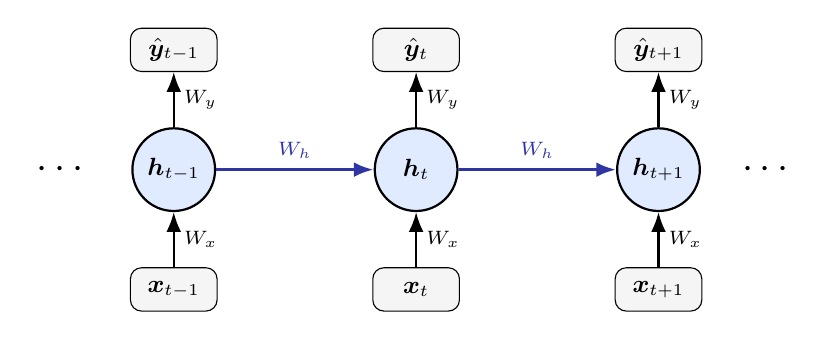
\begin{tikzpicture}[
    cell/.style={draw, circle, fill=SoftBlue, minimum size=1.05cm, font=\small, thick},
    io/.style={draw, rounded corners, fill=SoftGray, minimum width=1.1cm,
               minimum height=0.55cm, font=\small},
    arr/.style={-{Latex[length=2.5mm]}, thick},
    node distance=0.65cm and 2.0cm
]
\node[cell] (h1) {$\bm{h}_{t-1}$};
\node[cell, right=of h1] (h2) {$\bm{h}_t$};
\node[cell, right=of h2] (h3) {$\bm{h}_{t+1}$};

\node[io, below=0.7cm of h1] (x1) {$\bm{x}_{t-1}$};
\node[io, below=0.7cm of h2] (x2) {$\bm{x}_t$};
\node[io, below=0.7cm of h3] (x3) {$\bm{x}_{t+1}$};

\node[io, above=0.7cm of h1] (y1) {$\hat{\bm{y}}_{t-1}$};
\node[io, above=0.7cm of h2] (y2) {$\hat{\bm{y}}_t$};
\node[io, above=0.7cm of h3] (y3) {$\hat{\bm{y}}_{t+1}$};

\draw[arr] (x1) -- node[right,font=\scriptsize]{$W_x$} (h1);
\draw[arr] (x2) -- node[right,font=\scriptsize]{$W_x$} (h2);
\draw[arr] (x3) -- node[right,font=\scriptsize]{$W_x$} (h3);
\draw[arr] (h1) -- node[right,font=\scriptsize]{$W_y$} (y1);
\draw[arr] (h2) -- node[right,font=\scriptsize]{$W_y$} (y2);
\draw[arr] (h3) -- node[right,font=\scriptsize]{$W_y$} (y3);
\draw[arr, CourseBlue, very thick]
    (h1) -- node[above,font=\scriptsize,CourseBlue]{$W_h$} (h2);
\draw[arr, CourseBlue, very thick]
    (h2) -- node[above,font=\scriptsize,CourseBlue]{$W_h$} (h3);

\node[font=\Large, left=0.4cm of h1] {$\cdots$};
\node[font=\Large, right=0.4cm of h3] {$\cdots$};
\end{tikzpicture}
\end{center}

\vspace{0.1cm}
\begin{block}{Unrolling reveals depth}
In the time direction, the unrolled RNN is effectively a very deep network ---
with one layer per time step, all sharing the same weights $W_h$ and $W_x$.
Training this network requires differentiating through all layers simultaneously:
\textbf{Backpropagation Through Time}.
\end{block}
\end{frame}
%
%..................................................................
%
\begin{frame}{From Feedforward to Recurrent: Adding Memory}
\small
A feedforward network computes $\hat{y} = f(\bm{x})$: no memory between inputs.

\vspace{0.15cm}
A \textbf{recurrent neural network} (RNN) maintains a \textbf{hidden state}
$\bm{h}_t \in \R^n$ updated at every step:

\[
\boxed{
\bm{h}_t = \tanh\,\bigl(W_h\,\bm{h}_{t-1} + W_x\,\bm{x}_t + \bm{b}_h\bigr),
\qquad
\hat{\bm{y}}_t = \text{softmax}(W_y\,\bm{h}_t + \bm{b}_y).
}
\]

\vspace{0.1cm}
\begin{columns}[T]
\begin{column}{0.50\textwidth}
\begin{itemize}
    \item $\bm{x}_t \in \R^d$: current input (word embedding).
    \item $\bm{h}_{t-1} \in \R^n$: previous hidden state.
    \item $W_x \in \R^{n \times d}$, $W_h \in \R^{n \times n}$, $\bm{b}_h \in \R^n$: parameters.
    \item $\bm{h}_0 = \bm{0}$ by convention.
\end{itemize}
\end{column}
\begin{column}{0.46\textwidth}
\begin{alertblock}{Parameter sharing}
$W_h$, $W_x$, $W_y$ are \textbf{reused at every time step}.
This is what makes an RNN applicable to sequences of any length with a fixed parameter count.
\end{alertblock}
\end{column}
\end{columns}

\vspace{0.1cm}
\begin{block}{Interpretation of $\bm{h}_t$}
The hidden state is a \textbf{running summary} of all tokens $\bm{x}_1, \ldots, \bm{x}_t$.
It is the network's working memory of the sequence seen so far.
\end{block}
\end{frame}
%
%..................................................................
%
\begin{frame}{Recurrent Neural Network\enspace—\enspace Step $t=1$}
\centering
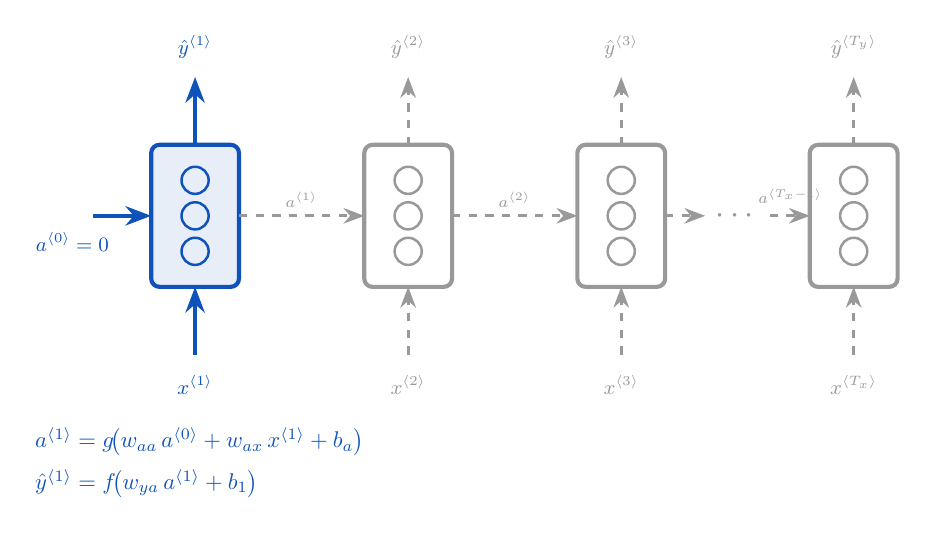
\begin{tikzpicture}[>=Stealth, scale=0.82, transform shape]

  %% ── Cells ─────────────────────────────────────────────────────
  \drawcell{ 0.0}{0}{actC }{actFill}   % t=1  ACTIVE
  \drawcell{ 3.3}{0}{futC }{white}     % t=2  future
  \drawcell{ 6.6}{0}{futC }{white}     % t=3  future
  \drawcell{10.2}{0}{futC }{white}     % t=Tx future

  %% ── ŷ labels (above cells) ────────────────────────────────────
  \node[color=actC,  font=\small] at ( 0.0, 2.62) {$\hat{y}^{\langle 1\rangle}$};
  \node[color=futC,  font=\small] at ( 3.3, 2.62) {$\hat{y}^{\langle 2\rangle}$};
  \node[color=futC,  font=\small] at ( 6.6, 2.62) {$\hat{y}^{\langle 3\rangle}$};
  \node[color=futC,  font=\small] at (10.2, 2.62) {$\hat{y}^{\langle T_y\rangle}$};

  %% ── x labels (below cells) ────────────────────────────────────
  \node[color=actC,  font=\small] at ( 0.0,-2.62) {$x^{\langle 1\rangle}$};
  \node[color=futC,  font=\small] at ( 3.3,-2.62) {$x^{\langle 2\rangle}$};
  \node[color=futC,  font=\small] at ( 6.6,-2.62) {$x^{\langle 3\rangle}$};
  \node[color=futC,  font=\small] at (10.2,-2.62) {$x^{\langle T_x\rangle}$};

  %% ── Dots ──────────────────────────────────────────────────────
  \node[color=futC, font=\Large] at (8.4, 0) {$\cdots$};

  %% ── a^{<0>} label ─────────────────────────────────────────────
  \node[color=actC, font=\small] at (-1.90, -0.40) {$a^{\langle 0\rangle} = 0$};

  %% ── Horizontal arrows (hidden-state flow) ─────────────────────
  % a^{<0>} → cell1   [active]
  \draw[->, color=actC,  line width=1.4pt]
    (-1.58, 0) -- (-0.68, 0);
  % cell1 → cell2    [future, dashed]
  \draw[->, color=futC,  line width=1.0pt, dashed]
    (0.68, 0) -- (2.62, 0);
  \node[color=futC,  font=\scriptsize, above] at (1.65, 0)
    {$a^{\langle 1\rangle}$};
  % cell2 → cell3    [future, dashed]
  \draw[->, color=futC,  line width=1.0pt, dashed]
    (3.98, 0) -- (5.92, 0);
  \node[color=futC,  font=\scriptsize, above] at (4.95, 0)
    {$a^{\langle 2\rangle}$};
  % cell3 → dots
  \draw[->, color=futC,  line width=1.0pt, dashed]
    (7.28, 0) -- (7.90, 0);
  % dots → cellTx
  \draw[->, color=futC,  line width=1.0pt, dashed]
    (8.90, 0) -- (9.52, 0);
  \node[color=futC,  font=\scriptsize, above] at (9.22, 0.06)
    {$a^{\langle T_x-1\rangle}$};

  %% ── Vertical input arrows (x → cell) ─────────────────────────
  \draw[->, color=actC,  line width=1.4pt]           ( 0.0,-2.15) -- ( 0.0,-1.10);
  \draw[->, color=futC,  line width=1.0pt, dashed]   ( 3.3,-2.15) -- ( 3.3,-1.10);
  \draw[->, color=futC,  line width=1.0pt, dashed]   ( 6.6,-2.15) -- ( 6.6,-1.10);
  \draw[->, color=futC,  line width=1.0pt, dashed]   (10.2,-2.15) -- (10.2,-1.10);

  %% ── Vertical output arrows (cell → ŷ) ────────────────────────
  \draw[->, color=actC,  line width=1.4pt]           ( 0.0, 1.10) -- ( 0.0, 2.15);
  \draw[->, color=futC,  line width=1.0pt, dashed]   ( 3.3, 1.10) -- ( 3.3, 2.15);
  \draw[->, color=futC,  line width=1.0pt, dashed]   ( 6.6, 1.10) -- ( 6.6, 2.15);
  \draw[->, color=futC,  line width=1.0pt, dashed]   (10.2, 1.10) -- (10.2, 2.15);

  %% ── Equations ─────────────────────────────────────────────────
  % Right block: active step equations
  \node[anchor=west, align=left, font=\normalsize] at (-2.6,-3.82) {%
    \textcolor{actC}{$a^{\langle 1\rangle}
      = g\!\bigl(w_{aa}\,a^{\langle 0\rangle}
               + w_{ax}\,x^{\langle 1\rangle} + b_a\bigr)$}\\[5pt]
    \textcolor{actC}{$\hat{y}^{\langle 1\rangle}
      = f\!\bigl(w_{ya}\,a^{\langle 1\rangle} + b_1\bigr)$}
  };

\end{tikzpicture}
\end{frame}
%
%..................................................................
%
\begin{frame}{Recurrent Neural Network\enspace—\enspace Step $t=2$}
\centering
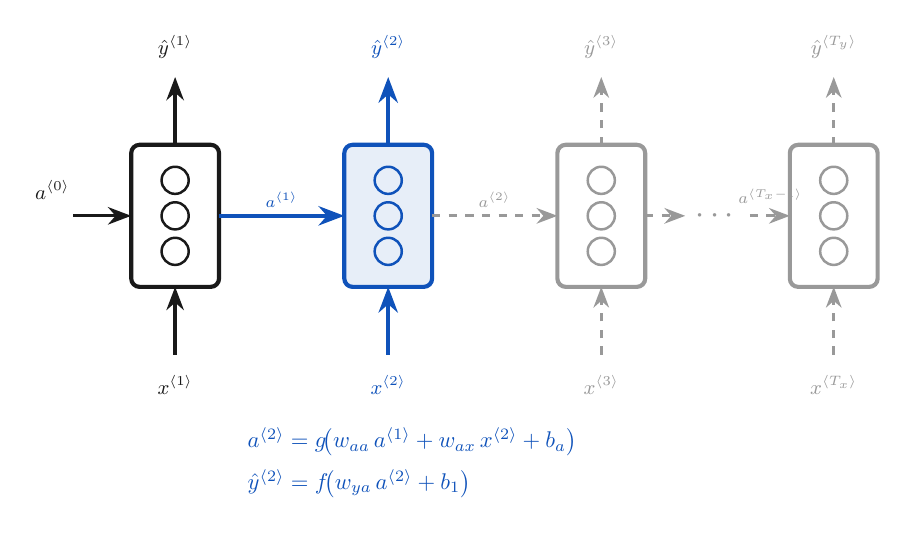
\begin{tikzpicture}[>=Stealth, scale=0.82, transform shape]

  %% ── Cells ─────────────────────────────────────────────────────
  \drawcell{ 0.0}{0}{doneC}{white}     % t=1  DONE
  \drawcell{ 3.3}{0}{actC }{actFill}   % t=2  ACTIVE
  \drawcell{ 6.6}{0}{futC }{white}     % t=3  future
  \drawcell{10.2}{0}{futC }{white}     % t=Tx future

  %% ── ŷ labels ──────────────────────────────────────────────────
  \node[color=doneC, font=\small] at ( 0.0, 2.62) {$\hat{y}^{\langle 1\rangle}$};
  \node[color=actC,  font=\small] at ( 3.3, 2.62) {$\hat{y}^{\langle 2\rangle}$};
  \node[color=futC,  font=\small] at ( 6.6, 2.62) {$\hat{y}^{\langle 3\rangle}$};
  \node[color=futC,  font=\small] at (10.2, 2.62) {$\hat{y}^{\langle T_y\rangle}$};

  %% ── x labels ──────────────────────────────────────────────────
  \node[color=doneC, font=\small] at ( 0.0,-2.62) {$x^{\langle 1\rangle}$};
  \node[color=actC,  font=\small] at ( 3.3,-2.62) {$x^{\langle 2\rangle}$};
  \node[color=futC,  font=\small] at ( 6.6,-2.62) {$x^{\langle 3\rangle}$};
  \node[color=futC,  font=\small] at (10.2,-2.62) {$x^{\langle T_x\rangle}$};

  %% ── Dots ──────────────────────────────────────────────────────
  \node[color=futC, font=\Large] at (8.4, 0) {$\cdots$};

  %% ── a^{<0>} label ─────────────────────────────────────────────
  \node[color=doneC, font=\small] at (-1.90, 0.40) {$a^{\langle 0\rangle}$};

  %% ── Horizontal arrows ─────────────────────────────────────────
  % a^{<0>} → cell1   [done]
  \draw[->, color=doneC, line width=1.2pt]
    (-1.58, 0) -- (-0.68, 0);
  % cell1 → cell2   [active: carries computed a^{<1>}]
  \draw[->, color=actC,  line width=1.4pt]
    (0.68, 0) -- (2.62, 0);
  \node[color=actC,  font=\scriptsize, above] at (1.65, 0)
    {$a^{\langle 1\rangle}$};
  % cell2 → cell3   [future, dashed]
  \draw[->, color=futC,  line width=1.0pt, dashed]
    (3.98, 0) -- (5.92, 0);
  \node[color=futC,  font=\scriptsize, above] at (4.95, 0)
    {$a^{\langle 2\rangle}$};
  % cell3 → dots
  \draw[->, color=futC,  line width=1.0pt, dashed]
    (7.28, 0) -- (7.90, 0);
  % dots → cellTx
  \draw[->, color=futC,  line width=1.0pt, dashed]
    (8.90, 0) -- (9.52, 0);
  \node[color=futC,  font=\scriptsize, above] at (9.22, 0.06)
    {$a^{\langle T_x-1\rangle}$};

  %% ── Vertical input arrows ─────────────────────────────────────
  \draw[->, color=doneC, line width=1.2pt]           ( 0.0,-2.15) -- ( 0.0,-1.10);
  \draw[->, color=actC,  line width=1.4pt]           ( 3.3,-2.15) -- ( 3.3,-1.10);
  \draw[->, color=futC,  line width=1.0pt, dashed]   ( 6.6,-2.15) -- ( 6.6,-1.10);
  \draw[->, color=futC,  line width=1.0pt, dashed]   (10.2,-2.15) -- (10.2,-1.10);

  %% ── Vertical output arrows ────────────────────────────────────
  \draw[->, color=doneC, line width=1.2pt]           ( 0.0, 1.10) -- ( 0.0, 2.15);
  \draw[->, color=actC,  line width=1.4pt]           ( 3.3, 1.10) -- ( 3.3, 2.15);
  \draw[->, color=futC,  line width=1.0pt, dashed]   ( 6.6, 1.10) -- ( 6.6, 2.15);
  \draw[->, color=futC,  line width=1.0pt, dashed]   (10.2, 1.10) -- (10.2, 2.15);

  %% ── Equations ─────────────────────────────────────────────────
  % Left block: previous step (greyed out — already computed)
%  \node[anchor=west, align=left, font=\small] at (-1.6,-2.82) {%
%    \textcolor{futC}{$a^{\langle 1\rangle}
%      = g\!\bigl(w_{aa}\,a^{\langle 0\rangle}
%               + w_{ax}\,x^{\langle 1\rangle} + b_a\bigr)$}\\[5pt]
%    \textcolor{futC}{$\hat{y}^{\langle 1\rangle}
%      = f\!\bigl(w_{ya}\,a^{\langle 1\rangle} + b_1\bigr)$}
%  };
  % Right block: active step equations
  \node[anchor=west, align=left, font=\normalsize] at (1.0,-3.82) {%
    \textcolor{actC}{$a^{\langle 2\rangle}
      = g\!\bigl(w_{aa}\,a^{\langle 1\rangle}
               + w_{ax}\,x^{\langle 2\rangle} + b_a\bigr)$}\\[5pt]
    \textcolor{actC}{$\hat{y}^{\langle 2\rangle}
      = f\!\bigl(w_{ya}\,a^{\langle 2\rangle} + b_1\bigr)$}
  };

\end{tikzpicture}
\end{frame}
%
%..................................................................
%
\begin{frame}{Recurrent Neural Network\enspace—\enspace Step $t=3$}
\centering
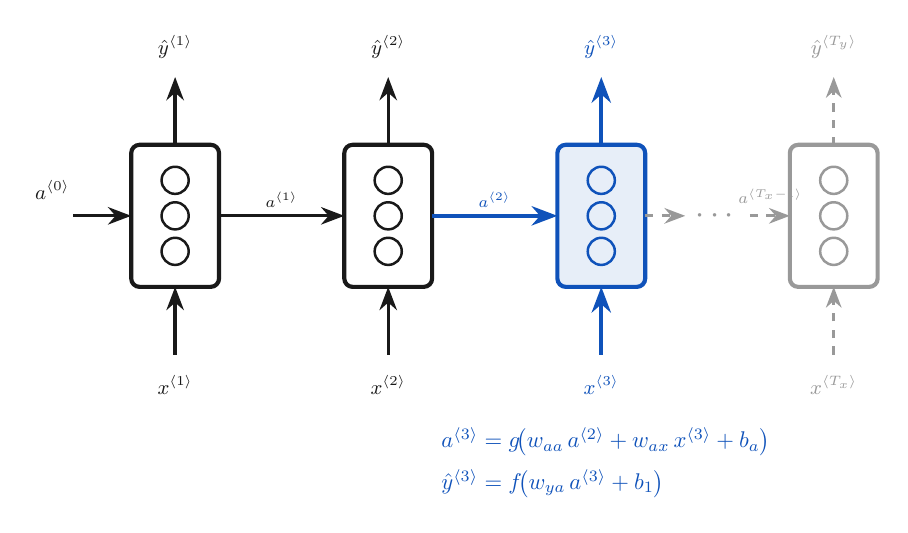
\begin{tikzpicture}[>=Stealth, scale=0.82, transform shape]

  %% ── Cells ─────────────────────────────────────────────────────
  \drawcell{ 0.0}{0}{doneC}{white}     % t=1  DONE
  \drawcell{ 3.3}{0}{doneC}{white}     % t=2  DONE
  \drawcell{ 6.6}{0}{actC }{actFill}   % t=3  ACTIVE
  \drawcell{10.2}{0}{futC }{white}     % t=Tx future

  %% ── ŷ labels ──────────────────────────────────────────────────
  \node[color=doneC, font=\small] at ( 0.0, 2.62) {$\hat{y}^{\langle 1\rangle}$};
  \node[color=doneC, font=\small] at ( 3.3, 2.62) {$\hat{y}^{\langle 2\rangle}$};
  \node[color=actC,  font=\small] at ( 6.6, 2.62) {$\hat{y}^{\langle 3\rangle}$};
  \node[color=futC,  font=\small] at (10.2, 2.62) {$\hat{y}^{\langle T_y\rangle}$};

  %% ── x labels ──────────────────────────────────────────────────
  \node[color=doneC, font=\small] at ( 0.0,-2.62) {$x^{\langle 1\rangle}$};
  \node[color=doneC, font=\small] at ( 3.3,-2.62) {$x^{\langle 2\rangle}$};
  \node[color=actC,  font=\small] at ( 6.6,-2.62) {$x^{\langle 3\rangle}$};
  \node[color=futC,  font=\small] at (10.2,-2.62) {$x^{\langle T_x\rangle}$};

  %% ── Dots ──────────────────────────────────────────────────────
  \node[color=futC, font=\Large] at (8.4, 0) {$\cdots$};

  %% ── a^{<0>} label ─────────────────────────────────────────────
  \node[color=doneC, font=\small] at (-1.90, 0.40) {$a^{\langle 0\rangle}$};

  %% ── Horizontal arrows ─────────────────────────────────────────
  % a^{<0>} → cell1   [done]
  \draw[->, color=doneC, line width=1.2pt]
    (-1.58, 0) -- (-0.68, 0);
  % cell1 → cell2   [done]
  \draw[->, color=doneC, line width=1.2pt]
    (0.68, 0) -- (2.62, 0);
  \node[color=doneC, font=\scriptsize, above] at (1.65, 0)
    {$a^{\langle 1\rangle}$};
  % cell2 → cell3   [active: carries computed a^{<2>}]
  \draw[->, color=actC,  line width=1.4pt]
    (3.98, 0) -- (5.92, 0);
  \node[color=actC,  font=\scriptsize, above] at (4.95, 0)
    {$a^{\langle 2\rangle}$};
  % cell3 → dots   [future, dashed]
  \draw[->, color=futC,  line width=1.0pt, dashed]
    (7.28, 0) -- (7.90, 0);
  % dots → cellTx
  \draw[->, color=futC,  line width=1.0pt, dashed]
    (8.90, 0) -- (9.52, 0);
  \node[color=futC,  font=\scriptsize, above] at (9.22, 0.06)
    {$a^{\langle T_x-1\rangle}$};

  %% ── Vertical input arrows ─────────────────────────────────────
  \draw[->, color=doneC, line width=1.2pt]           ( 0.0,-2.15) -- ( 0.0,-1.10);
  \draw[->, color=doneC, line width=1.2pt]           ( 3.3,-2.15) -- ( 3.3,-1.10);
  \draw[->, color=actC,  line width=1.4pt]           ( 6.6,-2.15) -- ( 6.6,-1.10);
  \draw[->, color=futC,  line width=1.0pt, dashed]   (10.2,-2.15) -- (10.2,-1.10);

  %% ── Vertical output arrows ────────────────────────────────────
  \draw[->, color=doneC, line width=1.2pt]           ( 0.0, 1.10) -- ( 0.0, 2.15);
  \draw[->, color=doneC, line width=1.2pt]           ( 3.3, 1.10) -- ( 3.3, 2.15);
  \draw[->, color=actC,  line width=1.4pt]           ( 6.6, 1.10) -- ( 6.6, 2.15);
  \draw[->, color=futC,  line width=1.0pt, dashed]   (10.2, 1.10) -- (10.2, 2.15);

  %% ── Equations ─────────────────────────────────────────────────
  % Left block: previous step (greyed out — already computed)
  %\node[anchor=west, align=left, font=\small] at (-1.6,-2.82) {%
%    \textcolor{futC}{$a^{\langle 2\rangle}
%      = g\!\bigl(w_{aa}\,a^{\langle 1\rangle}
%               + w_{ax}\,x^{\langle 2\rangle} + b_a\bigr)$}\\[5pt]
%    \textcolor{futC}{$\hat{y}^{\langle 2\rangle}
%      = f\!\bigl(w_{ya}\,a^{\langle 2\rangle} + b_1\bigr)$}
%  };
  % Right block: active step equations
  \node[anchor=west, align=left, font=\normalsize] at (4.0,-3.82) {%
    \textcolor{actC}{$a^{\langle 3\rangle}
      = g\!\bigl(w_{aa}\,a^{\langle 2\rangle}
               + w_{ax}\,x^{\langle 3\rangle} + b_a\bigr)$}\\[5pt]
    \textcolor{actC}{$\hat{y}^{\langle 3\rangle}
      = f\!\bigl(w_{ya}\,a^{\langle 3\rangle} + b_1\bigr)$}
  };

\end{tikzpicture}
\end{frame}
%
%..................................................................
%
\begin{frame}{Input-Output Configurations}
RNNs are flexible because the hidden state can be read out at any subset of time steps.

\vspace{0.15cm}
\begin{center}
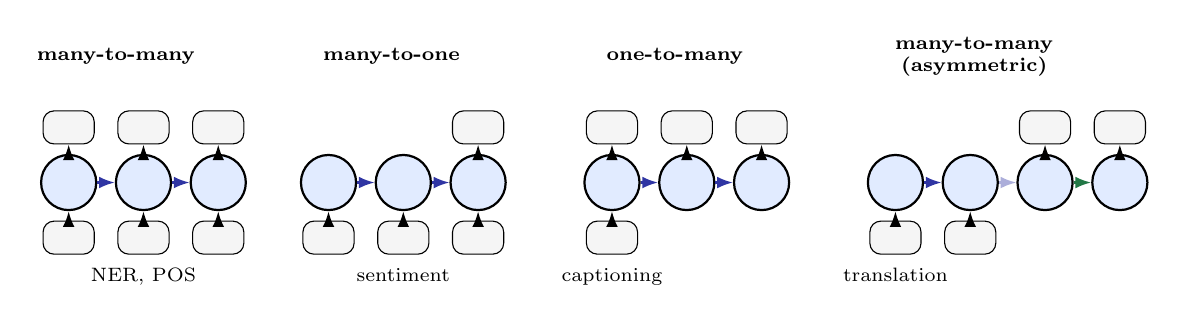
\begin{tikzpicture}[
    cell/.style={draw, circle, fill=SoftBlue, minimum size=0.7cm, font=\scriptsize, thick},
    io/.style={draw, rounded corners, fill=SoftGray, minimum width=0.65cm,
               minimum height=0.42cm, font=\scriptsize},
    arr/.style={-{Latex[length=2mm]}, thick},
    node distance=0.35cm and 0.9cm
]

% Many-to-many (same length)
\node[font=\scriptsize\bfseries] at (0.6, 1.6) {many-to-many};
\node[cell] (a1) at (0,0) {}; \node[cell] (a2) at (0.95,0) {}; \node[cell] (a3) at (1.9,0) {};
\node[io]   (ax1) at (0,-0.7) {}; \node[io] (ax2) at (0.95,-0.7) {}; \node[io] (ax3) at (1.9,-0.7) {};
\node[io]   (ay1) at (0,0.7) {};  \node[io] (ay2) at (0.95,0.7) {};  \node[io] (ay3) at (1.9,0.7) {};
\draw[arr,CourseBlue] (a1)--(a2); \draw[arr,CourseBlue] (a2)--(a3);
\draw[arr] (ax1)--(a1); \draw[arr] (ax2)--(a2); \draw[arr] (ax3)--(a3);
\draw[arr] (a1)--(ay1); \draw[arr] (a2)--(ay2); \draw[arr] (a3)--(ay3);
\node[font=\scriptsize, below=0.05cm of ax2] {NER, POS};

% Many-to-one
\node[font=\scriptsize\bfseries] at (4.1, 1.6) {many-to-one};
\node[cell] (b1) at (3.3,0) {}; \node[cell] (b2) at (4.25,0) {}; \node[cell] (b3) at (5.2,0) {};
\node[io]   (bx1) at (3.3,-0.7) {}; \node[io] (bx2) at (4.25,-0.7) {}; \node[io] (bx3) at (5.2,-0.7) {};
\node[io]   (by3) at (5.2,0.7) {};
\draw[arr,CourseBlue] (b1)--(b2); \draw[arr,CourseBlue] (b2)--(b3);
\draw[arr] (bx1)--(b1); \draw[arr] (bx2)--(b2); \draw[arr] (bx3)--(b3);
\draw[arr] (b3)--(by3);
\node[font=\scriptsize, below=0.05cm of bx2] {sentiment};

% One-to-many
\node[font=\scriptsize\bfseries] at (7.7, 1.6) {one-to-many};
\node[cell] (c1) at (6.9,0) {}; \node[cell] (c2) at (7.85,0) {}; \node[cell] (c3) at (8.8,0) {};
\node[io]   (cx1) at (6.9,-0.7) {};
\node[io]   (cy1) at (6.9,0.7) {};  \node[io] (cy2) at (7.85,0.7) {};  \node[io] (cy3) at (8.8,0.7) {};
\draw[arr,CourseBlue] (c1)--(c2); \draw[arr,CourseBlue] (c2)--(c3);
\draw[arr] (cx1)--(c1);
\draw[arr] (c1)--(cy1); \draw[arr] (c2)--(cy2); \draw[arr] (c3)--(cy3);
\node[font=\scriptsize, below=0.05cm of cx1] {captioning};

% Many-to-many different
\node[font=\scriptsize\bfseries,align=center] at (11.5, 1.6) {many-to-many\\(asymmetric)};
\node[cell] (d1) at (10.5,0) {}; \node[cell] (d2) at (11.45,0) {};
\node[cell] (d3) at (12.4,0) {}; \node[cell] (d4) at (13.35,0) {};
\node[io]   (dx1) at (10.5,-0.7) {}; \node[io] (dx2) at (11.45,-0.7) {};
\node[io]   (dy3) at (12.4,0.7) {};  \node[io] (dy4) at (13.35,0.7) {};
\draw[arr,CourseBlue] (d1)--(d2); \draw[arr,CourseBlue!40,dashed] (d2)--(d3); \draw[arr,Forest] (d3)--(d4);
\draw[arr] (dx1)--(d1); \draw[arr] (dx2)--(d2);
\draw[arr] (d3)--(dy3); \draw[arr] (d4)--(dy4);
\node[font=\scriptsize, below=0.05cm of dx1] {translation};
\end{tikzpicture}
\end{center}

\vspace{0.1cm}
\begin{alertblock}{The asymmetric many-to-many case}
When input and output have \textbf{different lengths}, a single RNN is not sufficient.
The model must first \textbf{encode} the entire input, then \textbf{decode} the output ---
the encoder-decoder architecture, the central topic of the second half of this lesson.
\end{alertblock}
\end{frame}
%
%..................................................................
%
\begin{frame}{Memory Cell}
\begin{columns}[T] % align columns
\begin{column}{.48\textwidth}
\textbf{Memory Cell}
\vspace{0.5cm}
        \begin{itemize}
		\item A memory cell refers to a fundamental component within an RNN unit that is designed to store and maintain information over time as the network processes sequential data.
		\item Memory cell is simply a different representation of the fundamental equations.
		\item Can be useful in order to understand the behaviour of more complex forms of recurrent network as GRU and LSTM.
        \end{itemize}
\end{column}%
\hfill%
\begin{column}{.48\textwidth}
    %\fbox{
        
\includegraphics[width=\linewidth]{../05-pictures/chapter-03_pic_1.png}
    %}
\end{column}%
\end{columns}
\end{frame}
%__________________________________________________________________________
%
\section{Backpropagation Through Time and the Vanishing Gradient}
%__________________________________________________________________________
%
\begin{frame}{Backpropagation Through Time: The Setup}
\small
For a sequence labeling task, the loss sums over time steps:
\[
\mathcal{L} = \sum_{t=1}^{T} \mathcal{L}_t.
\]

To update $W_h$ we need $\partial \mathcal{L} / \partial W_h$.
The contribution from $\mathcal{L}_t$ involves the gradient of $\bm{h}_t$
with respect to an \textbf{earlier} hidden state $\bm{h}_k$ ($k < t$):
\[
\frac{\partial \mathcal{L}_t}{\partial \bm{h}_k}
= \frac{\partial \mathcal{L}_t}{\partial \bm{h}_t}
  \cdot \prod_{j=k+1}^{t} \frac{\partial \bm{h}_j}{\partial \bm{h}_{j-1}}.
\]

The full gradient is then:
\[
\frac{\partial \mathcal{L}_t}{\partial W_h}
= \sum_{k=1}^{t}
  \frac{\partial \mathcal{L}_t}{\partial \bm{h}_t}
  \underbrace{\left(\prod_{j=k+1}^{t}
    W_h^{\!\top}\operatorname{diag}(\tanh'(z_j))
  \right)}_{\text{product of }(t-k)\text{ Jacobians}}
  \frac{\partial \bm{h}_k}{\partial W_h}.
\]
\end{frame}
%
%..................................................................
%
\begin{frame}{The Vanishing Gradient Problem}

The spectral norm of the product of Jacobians is bounded by:
\[
\left\|\prod_{j=k+1}^{t} W_h^{\!\top}\operatorname{diag}(\tanh'(z_j))\right\|
\;\leq\;
\lambda_{\max}(W_h)^{\,t-k},
\]
since $|\tanh'(z)| \leq 1$ for all $z$.

\vspace{0.15cm}
\begin{columns}[T]
\begin{column}{0.48\textwidth}
\begin{alertblock}{If $\lambda_{\max}(W_h) < 1$}
The product decays \textbf{exponentially} with $t - k$.
Gradients from distant steps vanish: the model cannot learn
long-range dependencies.
\emph{This is the vanishing gradient problem.}
\end{alertblock}
\end{column}
\begin{column}{0.48\textwidth}
\begin{alertblock}{If $\lambda_{\max}(W_h) > 1$}
The product \textbf{explodes} exponentially.
Training becomes numerically unstable.
\emph{This is the exploding gradient problem,}
addressed in practice by gradient clipping.
\end{alertblock}
\end{column}
\end{columns}
\end{frame}
%
%..................................................................
%
\begin{frame}{The Vanishing Gradient Problem}

\begin{center}
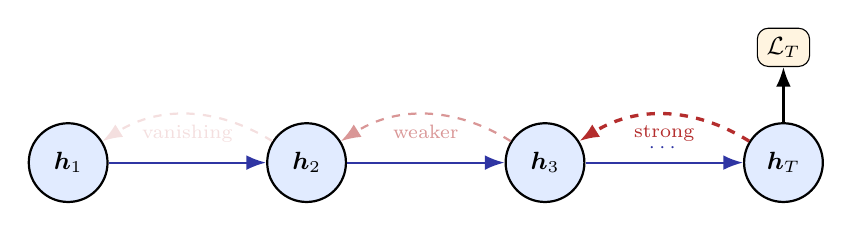
\begin{tikzpicture}[
    cell/.style={draw, circle, fill=SoftBlue, minimum size=1.0cm, font=\small, thick},
    io/.style={draw, rounded corners, fill=SoftGray, minimum width=1.0cm,
               minimum height=0.55cm, font=\small},
    arr/.style={-{Latex[length=2.5mm]}, thick},
    garr/.style={-{Latex[length=2.5mm]}, thick, dashed},
    node distance=0.6cm and 2.0cm
]
\node[cell] (h1) {$\bm{h}_1$};
\node[cell, right=of h1] (h2) {$\bm{h}_2$};
\node[cell, right=of h2] (h3) {$\bm{h}_3$};
\node[cell, right=of h3] (hT) {$\bm{h}_T$};

\draw[arr, CourseBlue] (h1) -- (h2);
\draw[arr, CourseBlue] (h2) -- (h3);
\draw[arr, CourseBlue] (h3) -- node[above,font=\scriptsize]{$\cdots$} (hT);

\node[draw, fill=SoftOrange, rounded corners, above=0.7cm of hT, font=\small] (L)
      {$\mathcal{L}_T$};
\draw[arr] (hT) -- (L);

\draw[garr, DeepRed, very thick]
    (hT) to[bend right=32] node[below,font=\scriptsize,DeepRed]{strong} (h3);
\draw[garr, DeepRed!50]
    (h3) to[bend right=32] node[below,font=\scriptsize,DeepRed!50]{weaker} (h2);
\draw[garr, DeepRed!15]
    (h2) to[bend right=32] node[below,font=\scriptsize,DeepRed!15]{vanishing} (h1);
\end{tikzpicture}
\end{center}

\vspace{0.15cm}
\begin{block}{Practical consequence}
A plain RNN has \textbf{effective memory of only a few steps}.
Information about the sentence beginning contributes negligible gradient
when computing $\partial \mathcal{L}_T / \partial W_h$ for large $T$.
\end{block}
\end{frame}
%
%..................................................................
%
\begin{frame}{The Vanishing Gradient Problem}
\small
\begin{center}
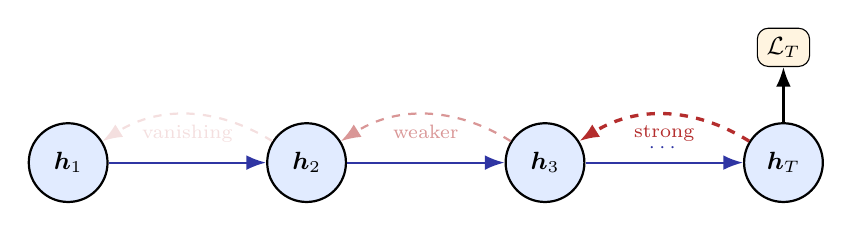
\begin{tikzpicture}[
    cell/.style={draw, circle, fill=SoftBlue, minimum size=1.0cm, font=\small, thick},
    io/.style={draw, rounded corners, fill=SoftGray, minimum width=1.0cm,
               minimum height=0.55cm, font=\small},
    arr/.style={-{Latex[length=2.5mm]}, thick},
    garr/.style={-{Latex[length=2.5mm]}, thick, dashed},
    node distance=0.6cm and 2.0cm
]
\node[cell] (h1) {$\bm{h}_1$};
\node[cell, right=of h1] (h2) {$\bm{h}_2$};
\node[cell, right=of h2] (h3) {$\bm{h}_3$};
\node[cell, right=of h3] (hT) {$\bm{h}_T$};

\draw[arr, CourseBlue] (h1) -- (h2);
\draw[arr, CourseBlue] (h2) -- (h3);
\draw[arr, CourseBlue] (h3) -- node[above,font=\scriptsize]{$\cdots$} (hT);

\node[draw, fill=SoftOrange, rounded corners, above=0.7cm of hT, font=\small] (L)
      {$\mathcal{L}_T$};
\draw[arr] (hT) -- (L);

\draw[garr, DeepRed, very thick]
    (hT) to[bend right=32] node[below,font=\scriptsize,DeepRed]{strong} (h3);
\draw[garr, DeepRed!50]
    (h3) to[bend right=32] node[below,font=\scriptsize,DeepRed!50]{weaker} (h2);
\draw[garr, DeepRed!15]
    (h2) to[bend right=32] node[below,font=\scriptsize,DeepRed!15]{vanishing} (h1);
\end{tikzpicture}
\end{center}

\begin{block}{Interpretation}
The gradient signal from $\mathcal{L}_T$ decays as it travels backwards through time.
By the time it reaches the first few steps, it carries almost no information.
Weights governing early steps receive \textbf{effectively zero update}.
\end{block}

\begin{alertblock}{The solution principle}
Redesign the recurrent cell so that the gradient has \textbf{a direct path back in time}
that does not pass through repeated matrix multiplications.
This is the core idea behind \textbf{gating mechanisms}.
\end{alertblock}
\end{frame}
%__________________________________________________________________________
%
\section{Gated Recurrent Units}
%__________________________________________________________________________
%
\begin{frame}{From Problem to Design Requirement}

The vanishing gradient is not a numerical accident. It follows directly from the structure of the
recurrent update. Recall the product of Jacobians accumulated over $t - k$ steps:

\[
  \frac{\partial \boldsymbol{h}_t}{\partial \boldsymbol{h}_k}
  = \prod_{j=k+1}^{t} \underbrace{W_h^{\top}\,\mathrm{diag}\!\bigl(\tanh'(z_j)\bigr)}_{\text{spectral norm} \;\leq\; \lambda_{\max}(W_h) < 1}
\]

Each factor shrinks the gradient signal. With $T - k$ steps, the product vanishes exponentially.

\medskip

\begin{block}{The design requirement}
We need $\partial \boldsymbol{h}_t / \partial \boldsymbol{h}_{t-1} \approx I$ in those dimensions where information
must survive across many steps.
The question is: \textbf{what recurrent update equation can produce a near-identity Jacobian
without freezing the network?}
\end{block}

\end{frame}
%
%..................................................................
%
\begin{frame}{Interpolation as the Solution (1/3)}

Define the \textbf{candidate state}
$\tilde{\boldsymbol{h}}_t = \tanh\!\bigl(W_h\,\boldsymbol{h}_{t-1} + W_x\,\boldsymbol{x}_t + \boldsymbol{b}\bigr)$
— the standard RNN nonlinear update. Consider two extreme ways of using it:

\bigskip
\begin{columns}[T]

  \begin{column}{0.46\textwidth}
    \begin{block}{Option 1 — Pure identity: $\boldsymbol{h}_t = \boldsymbol{h}_{t-1}$}
      The Jacobian is exactly the identity:
      \[
        \frac{\partial \boldsymbol{h}_t}{\partial \boldsymbol{h}_{t-1}} = I.
      \]
      Gradient never vanishes, regardless of sequence length.\\[4pt]
      \textbf{Problem:} the hidden state never changes — the network
      ignores all new input entirely. No learning is possible.
    \end{block}
  \end{column}

  \begin{column}{0.46\textwidth}
    \begin{alertblock}{Option 2 — Pure update: $\boldsymbol{h}_t = \tilde{\boldsymbol{h}}_t$}
      The Jacobian is the standard RNN factor:
      \[
        \frac{\partial \boldsymbol{h}_t}{\partial \boldsymbol{h}_{t-1}}
        = W_h^{\top}\mathrm{diag}\!\bigl(\tanh'(z_t)\bigr).
      \]
      \textbf{Problem:} spectral norm $\leq \lambda_{\max}(W_h) < 1$
      — the product over $t-k$ steps vanishes exponentially.
    \end{alertblock}
  \end{column}

\end{columns}

\end{frame}
%
%..................................................................
%
\begin{frame}{Interpolation as the Solution (2/3) — The Key Observation}
\small
\begin{block}{Option 1 — Pure identity}
  Gradient path is perfect, but the state is frozen: no information from $\boldsymbol{x}_t$ ever
  enters $\boldsymbol{h}_t$. The network cannot learn from new input.
\end{block}

\begin{alertblock}{Option 2 — Pure update}
  The network learns freely, but the Jacobian $W_h^{\top}\mathrm{diag}(\tanh'(z_t))$
  has spectral norm $< 1$: gradients from distant steps decay to zero.
\end{alertblock}
\normalsize
\begin{block}{The key observation}
  Neither extreme works. We need a \textbf{middle ground}: a mechanism that
  \emph{selectively} copies the past state in some dimensions (gradient $\approx 1$)
  while updating others (absorbing new input from $\boldsymbol{x}_t$),
  with the choice \emph{learned} at each step and dimension.\\[3pt]
  This is achieved by a \textbf{dimension-wise convex combination} — next slide.
\end{block}

\end{frame}
%
%..................................................................
%
\begin{frame}{Interpolation as the Solution (3/3)}

For $\boldsymbol{z} \in (0,1)^n$, form a \textbf{dimension-wise convex combination},
where $\boldsymbol{u} \odot \boldsymbol{v}$ denotes the \textbf{Hadamard product}
(element-wise multiplication: $(\boldsymbol{u} \odot \boldsymbol{v})_i = u_i v_i$):

\[
  \boldsymbol{h}_t \;=\;
  \underbrace{(1 - \boldsymbol{z})}_{\text{keep}} \odot \boldsymbol{h}_{t-1}
  \;+\;
  \underbrace{\boldsymbol{z}}_{\text{write}} \odot \tilde{\boldsymbol{h}}_t.
\]
The Jacobian w.r.t.\ $\boldsymbol{h}_{t-1}$ (direct path only) is:
\[
  \frac{\partial \boldsymbol{h}_t}{\partial \boldsymbol{h}_{t-1}}
  \;\approx\; \mathrm{diag}(1 - \boldsymbol{z}).
\]

\begin{alertblock}{Why this eliminates vanishing}
  \small
  Where $z_i \approx 0$: the Jacobian entry is $\approx 1$. No $W_h^{\top}$, no $\tanh'$,
  no exponential decay. Gradient flows unattenuated through those dimensions,
  for as many steps as $z_i$ remains small.
\end{alertblock}

\end{frame}
%
%..................................................................
%
\begin{frame}{How Is $\boldsymbol{z}$ Computed? Requirements}

For the convex combination $\boldsymbol{h}_t = (1-\boldsymbol{z})\odot\boldsymbol{h}_{t-1}
+ \boldsymbol{z}\odot\tilde{\boldsymbol{h}}_t$ to work, the coefficient $\boldsymbol{z}$
must satisfy two requirements:

\begin{columns}[T]

  \begin{column}{0.46\textwidth}
    \begin{block}{Requirement 1 — Range $(0,1)^n$}
      Each entry of $\boldsymbol{z}$ must be a valid interpolation weight,
      strictly between 0 and 1, so the combination is genuinely
      between identity and full update.\\[6pt]
      The \textbf{sigmoid} $\sigma(u) = 1/(1+e^{-u})$ maps any real
      input into $(0,1)$ element-wise — it is the natural choice.
    \end{block}
  \end{column}

  \begin{column}{0.46\textwidth}
    \begin{block}{Requirement 2 — Learned, context-aware}
      The network must decide \emph{when} to keep and \emph{when}
      to update, depending on both the current input $\boldsymbol{x}_t$
      and the accumulated state $\boldsymbol{h}_{t-1}$.\\[6pt]
      So $\boldsymbol{z}$ must be computed from
      $(\boldsymbol{h}_{t-1}, \boldsymbol{x}_t)$ through
      \textbf{trainable parameters}.
    \end{block}
  \end{column}

\end{columns}

\medskip
Both requirements are satisfied by a single equation:
\[
  \boldsymbol{z}_t \;=\; \sigma\!\bigl(W_z\,[\boldsymbol{h}_{t-1},\, \boldsymbol{x}_t] + \boldsymbol{b}_z\bigr).
\]

\end{frame}
%
%..................................................................
%
\begin{frame}{How Is $\boldsymbol{z}$ Computed? The Gate}

\begin{alertblock}{The gate}
  A \textbf{gate} is a sigmoid-computed interpolation coefficient $\boldsymbol{z}_t \in (0,1)^n$:
  \[
    \boldsymbol{z}_t = \sigma\!\bigl(W_z\,[\boldsymbol{h}_{t-1},\, \boldsymbol{x}_t] + \boldsymbol{b}_z\bigr).
  \]
  It steers the recurrent update dimension by dimension:
  \begin{itemize}
    \item $z_i \approx 1$: \textbf{write} — replace $h_{t-1,i}$ with the candidate $\tilde{h}_{t,i}$.
    \item $z_i \approx 0$: \textbf{keep} — copy $h_{t-1,i}$ unchanged;
      the direct gradient $\partial h_{t,i}/\partial h_{t-1,i} \approx 1$.
  \end{itemize}
\end{alertblock}

\medskip
\begin{block}{Why this solves the vanishing gradient}
  Where $z_i \approx 0$ across many steps, the Jacobian is near-identity in dimension $i$:
  no repeated multiplication by $W_h^{\top}$, no $\tanh'$ saturation, no exponential decay.
  Long-range gradients survive precisely because the gate \emph{learns} to keep them alive.
\end{block}

\end{frame}
%
%..................................................................
%
\begin{frame}{The Gating Idea}
\vspace{0.15cm}
\begin{block}{What gating achieves}
By learning to hold certain dimensions of $\bm{h}_t$ approximately constant
across many steps, a gated cell maintains a gradient path that is close to
\textbf{identity} in those dimensions --- bypassing the vanishing gradient.
\end{block}

\vspace{0.15cm}
The \textbf{Gated Recurrent Unit} (GRU, Cho et al.\ 2014) uses two gates:
\begin{columns}[T]
\begin{column}{0.48\textwidth}
\begin{itemize}
    \item \textbf{Update gate} $\bm{z}_t$: how much of the past state to retain.
\end{itemize}
\end{column}
\begin{column}{0.48\textwidth}
\begin{itemize}
    \item \textbf{Reset gate} $\bm{r}_t$: how much of the past state enters the candidate.
\end{itemize}
\end{column}
\end{columns}
\end{frame}
%
%..................................................................
%
\begin{frame}{GRU: Complete Equations}
\begin{columns}[T]
\begin{column}{0.50\textwidth}

\textbf{Step 1 --- Compute the gates}
\begin{align*}
\bm{z}_t &= \sigma(W_z\,[\bm{h}_{t-1},\,\bm{x}_t] + \bm{b}_z) \\[4pt]
\bm{r}_t &= \sigma(W_r\,[\bm{h}_{t-1},\,\bm{x}_t] + \bm{b}_r)
\end{align*}

\smallskip
\textbf{Step 2 --- Compute the candidate state}
\[
\tilde{\bm{h}}_t = \tanh\!\bigl(W_h\,[\bm{r}_t \odot \bm{h}_{t-1},\;\bm{x}_t] + \bm{b}_h\bigr)
\]

\smallskip
\textbf{Step 3 --- Interpolate old and new}
\[
\bm{h}_t = (1 - \bm{z}_t) \odot \bm{h}_{t-1} + \bm{z}_t \odot \tilde{\bm{h}}_t
\]

\end{column}
\begin{column}{0.46\textwidth}
\begin{block}{Reading the update equation}
\[
\bm{h}_t =
\underbrace{(1-\bm{z}_t)}_{\text{keep}} \odot \bm{h}_{t-1}
+
\underbrace{\bm{z}_t}_{\text{write}} \odot \tilde{\bm{h}}_t
\]
$\bm{z}_t \approx \bm{0}$: cell \textbf{copies} past state, no change.\\[4pt]
$\bm{z}_t \approx \bm{1}$: cell \textbf{replaces} with the candidate.
\end{block}

\begin{alertblock}{Gradient path}
When $\bm{z}_t \approx \bm{0}$ over several steps:
$\bm{h}_t \approx \bm{h}_{t-1}$, so
$\partial \bm{h}_t / \partial \bm{h}_{t-1} \approx I$.
No vanishing in those dimensions.
\end{alertblock}
\end{column}
\end{columns}
\end{frame}
%
%..................................................................
%
\begin{frame}{GRU: What Each Gate Does in Practice}
\begin{columns}[T]
\begin{column}{0.48\textwidth}
\begin{block}{Reset gate $\bm{r}_t$}
Controls how much of $\bm{h}_{t-1}$ is used to compute $\tilde{\bm{h}}_t$.

\smallskip
When $\bm{r}_t \approx \bm{0}$: the candidate ignores the past and focuses only on $\bm{x}_t$.

\smallskip
\textbf{Example:} In \emph{``\ldots after a long digression, \textbf{the main thesis} is\ldots''}
the reset gate allows the model to partially discard the digression when processing the final clause.
\end{block}
\end{column}
\begin{column}{0.48\textwidth}
\begin{block}{Update gate $\bm{z}_t$}
Controls the interpolation between old and new state.

\smallskip
When $\bm{z}_t \approx \bm{0}$: the hidden state is \textbf{preserved unchanged}.
This is how long-range information survives.

\smallskip
\textbf{Example:} The subject of a long subordinate clause is kept alive in $\bm{h}_t$
until the main verb is finally read.
\end{block}
\end{column}
\end{columns}

%\vspace{0.2cm}
%\begin{block}{A single learnable interpolation}
%Unlike LSTM, GRU merges the ``forget'' and ``input'' decisions into a single gate $\bm{z}_t$:
%remembering more of the past ($1 - \bm{z}_t$ large) automatically means writing less of the candidate.
%\end{block}
\end{frame}
%__________________________________________________________________________
%
\section{Long Short-Term Memory}
%__________________________________________________________________________
%
\begin{frame}{From GRU to LSTM: Why a Separate Memory?}

The GRU solves the vanishing gradient with a single state vector
$\vct{h}_t$ that doubles as both \textbf{long-term memory} and
\textbf{output to the next layer}.

\begin{block}{A limitation of this design}
Every dimension of $\vct{h}_t$ that is \emph{kept} unchanged
(gate $z_i \approx 0$) is also exposed as output.  Conversely,
every dimension that is \emph{overwritten} to produce a useful
output is lost from memory.

The network cannot simultaneously \textbf{remember} something
and \textbf{choose not to expose} it at the current step.
\end{block}

\begin{alertblock}{The LSTM insight (Hochreiter \& Schmidhuber, 1997)}
Decouple the two roles: maintain a dedicated \textbf{cell state}
$\vct{c}_t$ for long-term storage, and a separate \textbf{hidden
state} $\vct{h}_t$ for output.  The cell state is the network's
private notebook; the hidden state is what it chooses to say aloud.
\end{alertblock}

\end{frame}
%
%..................................................................
%
\begin{frame}{Decoupling Storage from Output}

\begin{columns}[T]
\begin{column}{0.48\textwidth}

\begin{block}{GRU: single state}
$\vct{h}_t$ is both memory and output.

\medskip
\begin{itemize}
\item Keep a dimension $\Rightarrow$ it is also exposed.
\item Overwrite a dimension $\Rightarrow$ old information is lost.
\end{itemize}

\medskip
Two competing uses, one vector.
\end{block}

\end{column}
\begin{column}{0.48\textwidth}

\begin{block}{LSTM: two state vectors}
$\vct{c}_t$: cell state --- long-term storage.\\
$\vct{h}_t$: hidden state --- current output.

\medskip
\begin{itemize}
\item The cell can hold information for hundreds of
      steps without ever exposing it.
\item The output gate controls which parts of
      $\vct{c}_t$ appear in $\vct{h}_t$ at each step.
\end{itemize}
\end{block}

\end{column}
\end{columns}
\end{frame}
%
%..................................................................
%
\begin{frame}{Decoupling Storage from Output}

\begin{alertblock}{An analogy}
Consider reading a detective novel.  Your memory retains clues from
chapter~1 (cell state), but you do not reveal the solution until the
final chapter (output gate).  The GRU must either reveal or forget;
the LSTM can silently carry information forward and expose it only
when needed.
\end{alertblock}

\end{frame}
%
%..................................................................
%
\begin{frame}{The LSTM Cell: A Guided Tour}
\begin{center}

\includegraphics[scale=.35]{../05-pictures/chapter-03_pic_2.png} 
\end{center}
\end{frame}
%
%..................................................................
%
\begin{frame}{The LSTM Cell: A Guided Tour}

The LSTM update proceeds in three phases, each controlled by a
learned gate:

\bigskip

\begin{columns}[T]
\begin{column}{0.32\textwidth}
\centering
\textcolor{red!70!black}{\textbf{Phase 1 --- Forget}}

\medskip
\fbox{$\vct{f}_t = \sigma\!\bigl(W_f[\vct{h}_{t-1}, \vct{x}_t]
      + \vct{b}_f\bigr)$}

\medskip
\small
Decide which dimensions of $\vct{c}_{t-1}$ are no longer relevant.

$f_i \approx 0$: erase dimension $i$.\\
$f_i \approx 1$: retain it.
\end{column}

\begin{column}{0.32\textwidth}
\centering
\textcolor{green!50!black}{\textbf{Phase 2 --- Write}}

\medskip
\fbox{$\begin{aligned}
\vct{i}_t &= \sigma\!\bigl(W_i[\vct{h}_{t-1}, \vct{x}_t]
             + \vct{b}_i\bigr)\\
\tilde{\vct{c}}_t &= \tanh\!\bigl(W_c[\vct{h}_{t-1}, \vct{x}_t]
             + \vct{b}_c\bigr)
\end{aligned}$}

\medskip
\small
Compute a candidate $\tilde{\vct{c}}_t$ and gate it by~$\vct{i}_t$
to decide \emph{what} and \emph{how much} to write.
\end{column}

\begin{column}{0.32\textwidth}
\centering
\textcolor{blue!70!black}{\textbf{Phase 3 --- Read out}}

\medskip
\fbox{$\begin{aligned}
\vct{o}_t &= \sigma\!\bigl(W_o[\vct{h}_{t-1}, \vct{x}_t]
             + \vct{b}_o\bigr)\\
\vct{h}_t &= \vct{o}_t \odot \tanh(\vct{c}_t)
\end{aligned}$}

\medskip
\small
The output gate selects which parts of the updated cell state are
exposed as the hidden state $\vct{h}_t$.
\end{column}

\end{columns}
\end{frame}
%
%..................................................................
%
\begin{frame}{The LSTM Cell: A Guided Tour}

\begin{alertblock}{The cell update in one line}
\[
\vct{c}_t
  = \underbrace{\vct{f}_t \odot \vct{c}_{t-1}}_{\text{selectively forget}}
  + \underbrace{\vct{i}_t \odot \tilde{\vct{c}}_t}_{\text{selectively write}}
\]
No $W_h^\top$, no $\tanh'$ on the recurrent path --- just
element-wise scaling by $\vct{f}_t \in (0,1)^n$.
\end{alertblock}

\end{frame}
%
%..................................................................
%
\begin{frame}{LSTM: The Four Gate Equations}

All gates take $[\bm{h}_{t-1},\, \bm{x}_t]$ as input.

\vspace{0.1cm}
\begin{columns}[T]
\begin{column}{0.50\textwidth}
\footnotesize
{\color{GateOrange}\textbf{Forget gate}} --- what to erase from $\bm{c}_{t-1}$:
\[
\bm{f}_t = \sigma(W_f\,[\bm{h}_{t-1},\,\bm{x}_t] + \bm{b}_f)
\]

{\color{Forest}\textbf{Input gate}} + \textbf{candidate} --- what to write:
\begin{align*}
\bm{i}_t       &= \sigma(W_i\,[\bm{h}_{t-1},\,\bm{x}_t] + \bm{b}_i) \\
\tilde{\bm{c}}_t &= \tanh(W_c\,[\bm{h}_{t-1},\,\bm{x}_t] + \bm{b}_c)
\end{align*}

{\color{CellGold}\textbf{Cell state update}}:
\[
\bm{c}_t = \bm{f}_t \odot \bm{c}_{t-1} + \bm{i}_t \odot \tilde{\bm{c}}_t
\]

{\color{CourseBlue}\textbf{Output gate}} --- what to expose as $\bm{h}_t$:
\begin{align*}
\bm{o}_t &= \sigma(W_o\,[\bm{h}_{t-1},\,\bm{x}_t] + \bm{b}_o) \\
\bm{h}_t &= \bm{o}_t \odot \tanh(\bm{c}_t)
\end{align*}

\end{column}
\begin{column}{0.46\textwidth}
\vspace{-.75cm}
\normalsize
\begin{block}{The cell update in full}
\[
\bm{c}_t
= \underbrace{\bm{f}_t \odot \bm{c}_{t-1}}_{\text{selectively forget}}
+ \underbrace{\bm{i}_t \odot \tilde{\bm{c}}_t}_{\text{selectively write}}
\]
\end{block}

\begin{alertblock}{Why the gradient survives}
\[
\frac{\partial \bm{c}_t}{\partial \bm{c}_{t-1}} = \operatorname{diag}(\bm{f}_t)
\]
This is a \textbf{diagonal} matrix with entries in $(0,1)$.
No $\tanh'$, no $W_h^{\top}$.
The cell state gradient can flow back many steps
without collapsing.
\end{alertblock}

\end{column}
\end{columns}
\end{frame}
%
%..................................................................
%
\begin{frame}{LSTM: What Each Gate Does in Practice}

\small
\begin{columns}[T]
\begin{column}{0.48\textwidth}

\begin{block}{Forget gate $\vct{f}_t$}
Decides which dimensions of $\vct{c}_{t-1}$ to erase.
$f_i \approx 0$: erase; $f_i \approx 1$: retain.

\smallskip
\textbf{Example:} When a full stop is read, the forget gate clears
the subject and tense of the previous sentence, making room for the next.
\end{block}

\smallskip

\begin{block}{Input gate $\vct{i}_t$ + candidate $\tilde{\vct{c}}_t$}
The candidate proposes \emph{what} to write; the input gate decides
\emph{how much} of each dimension enters $\vct{c}_t$.

\smallskip
\textbf{Example:} Upon reading a new subject, the input gate opens
to store it; filler words are largely blocked.
\end{block}

\end{column}
\begin{column}{0.48\textwidth}

\begin{block}{Output gate $\vct{o}_t$}
Controls which parts of $\vct{c}_t$ are visible in $\vct{h}_t$
--- the vector passed to the next layer and the next time step.

$o_i \approx 0$: dimension $i$ is remembered but \textbf{not exposed}.

\smallskip
\textbf{Example:} A translation model may store grammatical gender
in $\vct{c}_t$ from the source sentence, but only expose it through
$\vct{h}_t$ when generating a gender-agreeing adjective.
\end{block}

\smallskip

%\begin{alertblock}{Why three gates, not two?}
%GRU ties forget and input into one gate ($z$ and $1\!-\!z$).
%LSTM decouples them: the cell can \emph{simultaneously} forget old
%and write new information in the \emph{same} dimension --- added
%flexibility that helps on tasks with complex, overlapping dependencies.
%\end{alertblock}
\end{column}
\end{columns}
\end{frame}
%
%..................................................................
%
\begin{frame}{The LSTM Gradient Highway}

The gradient of the loss w.r.t.\ an earlier cell state $\vct{c}_k$
passes through a product of diagonal matrices:
\[
\frac{\partial \vct{c}_t}{\partial \vct{c}_k}
  = \prod_{j=k+1}^{t} \operatorname{diag}(\vct{f}_j).
\]

Compare with the plain RNN:
\[
\frac{\partial \vct{h}_t}{\partial \vct{h}_k}
  = \prod_{j=k+1}^{t}
    W_h^\top \operatorname{diag}\!\bigl(\tanh'(z_j)\bigr).
\]
\vspace{-.3cm}
\begin{alertblock}{Why LSTM wins}
\begin{itemize}\setlength{\itemsep}{1pt}
\item No weight matrix $W_h^\top$ --- only element-wise scaling.
\item No $\tanh'$ saturation --- forget gate values are in $(0,1)$.
\item When $f_i \!\approx\! 1$ across many steps:
      $\partial c_{t,i}/\partial c_{k,i} \approx 1$.
      Gradient flows back \textbf{unattenuated}.
\end{itemize}
\end{alertblock}

\end{frame}
%
%..................................................................
%
\begin{frame}{The LSTM Gradient Highway}
\begin{center}
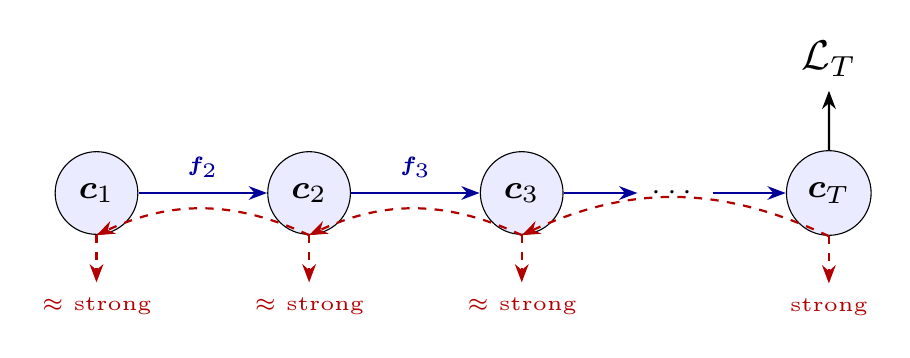
\begin{tikzpicture}[
    >=Stealth,
    cell/.style={draw, circle, minimum size=0.7cm, fill=blue!8,
                 font=\footnotesize},
    arr/.style={->, thick},
    garr/.style={->, thick, dashed, red!70!black},
    scale=1.5, transform shape
]

% cells
\node[cell] (c1) at (0,0) {$\vct{c}_1$};
\node[cell] (c2) at (1.8,0) {$\vct{c}_2$};
\node[cell] (c3) at (3.6,0) {$\vct{c}_3$};
\node[font=\scriptsize] (dots) at (4.9,0) {$\cdots$};
\node[cell] (cT) at (6.2,0) {$\vct{c}_T$};

% forward arrows
\draw[arr, blue!60!black] (c1) -- node[above, font=\tiny]
    {$\vct{f}_2$} (c2);
\draw[arr, blue!60!black] (c2) -- node[above, font=\tiny]
    {$\vct{f}_3$} (c3);
\draw[arr, blue!60!black] (c3) -- (dots);
\draw[arr, blue!60!black] (dots) -- (cT);

% loss
\node[above=0.5cm of cT] (L) {$\mathcal{L}_T$};
\draw[arr] (cT) -- (L);

% gradient arrows (backward, under the cells)
\draw[garr] (cT.south) -- ++(0, -0.4)
    node[below, font=\tiny, text=red!70!black]{strong};
\draw[garr] (c3.south) -- ++(0, -0.4)
    node[below, font=\tiny, text=red!70!black]{$\approx$ strong};
\draw[garr] (c2.south) -- ++(0, -0.4)
    node[below, font=\tiny, text=red!70!black]{$\approx$ strong};
\draw[garr] (c1.south) -- ++(0, -0.4)
    node[below, font=\tiny, text=red!70!black]{$\approx$ strong};

% backward path
\draw[garr, bend right=25] (cT.south) to (c3.south);
\draw[garr, bend right=25] (c3.south) to (c2.south);
\draw[garr, bend right=25] (c2.south) to (c1.south);

\end{tikzpicture}
\end{center}

\smallskip
When the forget gate keeps $f_i \!\approx\! 1$, the gradient signal from
$\mathcal{L}_T$ reaches $\vct{c}_1$ at nearly full strength --- contrast
with the exponential decay in a plain RNN (slide~30).

\smallskip
The network \emph{learns} which dimensions to protect: the forget gate
is trained, not hand-tuned.
\end{frame}
%
%..................................................................
%
\begin{frame}{GRU versus LSTM: Comparison}
\vspace{0.15cm}
\begin{block}{Practical guidance}
In modern NLP the choice between GRU and LSTM is often secondary to architecture and data scale.
Both have been largely superseded by transformers for language tasks,
but they remain important baselines and are widely used in time-series applications.
\end{block}
\end{frame}
%__________________________________________________________________________
%
\section{Sequence-to-Sequence and the Encoder-Decoder Architecture}
%__________________________________________________________________________
%
\begin{frame}{The Seq2Seq Problem}
Many critical NLP tasks map an input sequence of \emph{one length} to an output
sequence of a \emph{different length}:
\begin{itemize}
    \item \textbf{Machine translation:}
          \emph{``The committee published its final report.''} $\to$
          \emph{``Il comitato ha pubblicato il suo rapporto finale.''}
    \item \textbf{Abstractive summarization:} a 400-word news article $\to$ a 3-sentence abstract.
    \item \textbf{Question answering:} question + long passage $\to$ a short answer.
    \item \textbf{Dialogue modeling:} a conversational turn $\to$ a coherent reply.
\end{itemize}
\end{frame}
%
%..................................................................
%
\begin{frame}{The Seq2Seq Problem}
\vspace{0.15cm}
\begin{block}{Why a single RNN is not sufficient}
A single RNN produces one output per input step.
For asymmetric lengths, we need to \textbf{read the entire input first} and
\textbf{generate the output second}.
These are distinct operations requiring distinct components.
\end{block}

\vspace{0.1cm}
The \textbf{encoder-decoder architecture} (Sutskever et al.\ 2014; Cho et al.\ 2014)
provides exactly this two-phase structure.
\end{frame}
%
%..................................................................
%
\begin{frame}{Encoder-Decoder: The Central Idea}
\small
The sequence-to-sequence problem is not only a problem of variable length. It is a problem of
\textbf{two different operations}.

\vspace{0.35cm}
\begin{columns}[T,onlytextwidth]
\column{0.48\textwidth}
\begin{block}{1. Encoding: read the source}
Given an input sequence
\[
  x_{1:T} = (x_1,x_2,\ldots,x_T),
\]
the encoder reads all source tokens and produces a compact representation of the input.
\end{block}

\column{0.48\textwidth}
\begin{block}{2. Decoding: generate the target}
Given the encoded representation, the decoder generates an output sequence
\[
  y_{1:S} = (y_1,y_2,\ldots,y_S),
\]
one token at a time.
\end{block}
\end{columns}

\vspace{0.25cm}
\begin{alertblock}{Key point}
The encoder-decoder architecture separates \textbf{understanding the source} from \textbf{producing the target}.
\end{alertblock}
\end{frame}
%
%..................................................................
%
\begin{frame}{The Two-Phase Computation}
\small
The architecture can be summarized as a two-phase computational pipeline:

\vspace{0.3cm}
\begin{center}
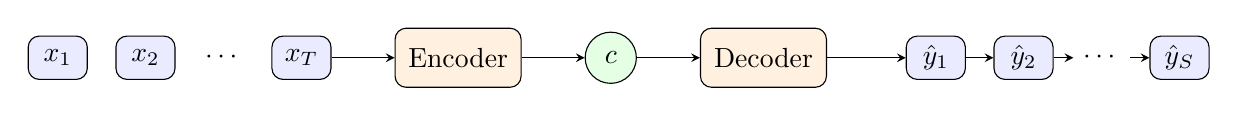
\begin{tikzpicture}[>=stealth, node distance=1.4cm]
  \tikzstyle{token}=[draw, rounded corners, minimum width=0.75cm, minimum height=0.55cm, fill=blue!8]
  \tikzstyle{state}=[draw, circle, minimum size=0.65cm, fill=green!10]
  \tikzstyle{box}=[draw, rounded corners, minimum width=1.6cm, minimum height=0.75cm, fill=orange!12]

  \node[token] (x1) {$x_1$};
  \node[token, right=0.35cm of x1] (x2) {$x_2$};
  \node[right=0.25cm of x2] (dotsx) {$\cdots$};
  \node[token, right=0.25cm of dotsx] (xT) {$x_T$};

  \node[box, right=0.8cm of xT] (enc) {Encoder};
  \node[state, right=0.8cm of enc] (c) {$c$};
  \node[box, right=0.8cm of c] (dec) {Decoder};

  \node[token, right=1.0cm of dec] (y1) {$\hat{y}_1$};
  \node[token, right=0.35cm of y1] (y2) {$\hat{y}_2$};
  \node[right=0.25cm of y2] (dotsy) {$\cdots$};
  \node[token, right=0.25cm of dotsy] (yS) {$\hat{y}_S$};

  \draw[->] (xT) -- (enc);
  \draw[->] (enc) -- (c);
  \draw[->] (c) -- (dec);
  \draw[->] (dec) -- (y1);
  \draw[->] (y1) -- (y2);
  \draw[->] (y2) -- (dotsy);
  \draw[->] (dotsy) -- (yS);
\end{tikzpicture}
\end{center}

\vspace{0.2cm}
Where:
\[
  x_t \in \mathbb{R}^{d_x} \quad \text{is the source-token embedding at position } t,
\]
\[
  y_s \quad \text{is the target token at position } s,
  \qquad c \in \mathbb{R}^{n} \quad \text{is the context vector.}
\]

\begin{alertblock}{Interpretation}
The vector $c$ is the bridge between the two phases: it is the output of the encoder and the conditioning information for the decoder.
\end{alertblock}
\end{frame}
%
%..................................................................
%
\begin{frame}{The Encoder: Compressing a Sequence into a Vector}
\small
The encoder is a recurrent network (LSTM or GRU) that reads
$\bm{x}_1, \ldots, \bm{x}_T$ and produces hidden states
$\bm{h}_1^{(e)}, \ldots, \bm{h}_T^{(e)}$.
Only the \textbf{final state} is passed forward as the \textbf{context vector}:
\[
\bm{c} = \bm{h}_T^{(e)} \;\in\; \R^n.
\]

\begin{center}
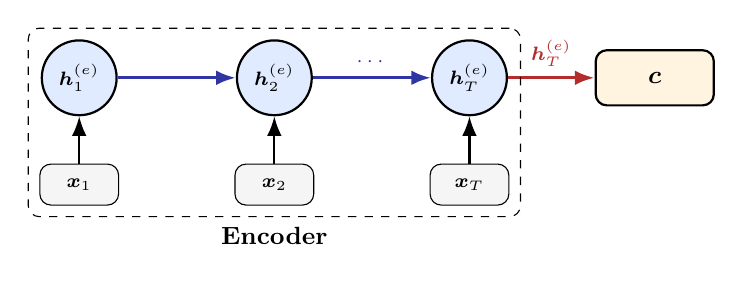
\begin{tikzpicture}[
    cell/.style={draw, circle, fill=SoftBlue, minimum size=0.95cm, font=\scriptsize, thick},
    io/.style={draw, rounded corners, fill=SoftGray, minimum width=1.0cm,
               minimum height=0.52cm, font=\scriptsize},
    ctx/.style={draw, rounded corners, fill=SoftOrange, minimum width=1.5cm,
                minimum height=0.7cm, font=\small, thick},
    arr/.style={-{Latex[length=2.5mm]}, thick},
    node distance=0.5cm and 1.5cm
]
\node[cell] (e1) {$\bm{h}_1^{(e)}$};
\node[cell, right=of e1] (e2) {$\bm{h}_2^{(e)}$};
\node[cell, right=of e2] (eT) {$\bm{h}_T^{(e)}$};
\node[io, below=0.6cm of e1] (x1) {$\bm{x}_1$};
\node[io, below=0.6cm of e2] (x2) {$\bm{x}_2$};
\node[io, below=0.6cm of eT] (xT) {$\bm{x}_T$};
\node[ctx, right=1.1cm of eT] (c) {$\bm{c}$};

\draw[arr] (x1) -- (e1);
\draw[arr] (x2) -- (e2);
\draw[arr] (xT) -- (eT);
\draw[arr, CourseBlue, very thick] (e1) -- (e2);
\draw[arr, CourseBlue, very thick] (e2) -- node[above,font=\scriptsize]{$\cdots$} (eT);
\draw[arr, DeepRed, very thick]
    (eT) -- node[above,font=\scriptsize,DeepRed]{$\bm{h}_T^{(e)}$} (c);

\node[draw, dashed, rounded corners, fit=(e1)(e2)(eT)(x1)(xT),
      inner sep=4pt, label=below:{\small\textbf{Encoder}}] {};
\end{tikzpicture}
\end{center}

\begin{block}{The compression task}
$\bm{c}$ must encode all relevant information from $\bm{x}_1, \ldots, \bm{x}_T$
into a fixed $n$-dimensional vector.
The encoder is trained end-to-end so that $\bm{c}$ contains
precisely what the decoder will need.
\end{block}
\end{frame}
%
%..................................................................
%
\begin{frame}{The Context Vector as a Learned Summary}
\small
Assume, for simplicity, an RNN encoder. The encoder hidden states are computed as
\[
  h^{(e)}_t = f_{\mathrm{enc}}\left(h^{(e)}_{t-1}, x_t\right),
  \qquad t=1,\ldots,T,
\]
where:
\begin{itemize}
  \item $h^{(e)}_t \in \mathbb{R}^{n}$ is the encoder hidden state after reading token $x_t$;
  \item $f_{\mathrm{enc}}$ is the recurrent update function, for example an RNN, GRU, or LSTM cell;
  \item $T$ is the source-sequence length.
\end{itemize}

\vspace{0.2cm}
The simplest encoder-decoder model defines the context vector as
\[
  c = h^{(e)}_T.
\]

\begin{block}{Meaning of $c$}
The vector $c$ is not hand-designed. It is a \textbf{learned summary} of the full source sequence $x_{1:T}$, optimized only because it helps the decoder predict the correct target sequence.
\end{block}
\end{frame}
%
%..................................................................
%
\begin{frame}{What Information Must the Context Vector Carry?}
\small
For machine translation, $c$ must contain whatever the decoder will need in order to generate the target sentence.

\vspace{0.25cm}
\begin{columns}[T,onlytextwidth]
\column{0.48\textwidth}
\begin{block}{Lexical information}
Which concepts and words appear in the source sentence?
\end{block}
\begin{block}{Syntactic information}
Who is the subject? What is the object? What modifies what?
\end{block}

\column{0.48\textwidth}
\begin{block}{Semantic information}
What situation or event is described by the sentence?
\end{block}
\begin{block}{Generation-relevant information}
Which tense, number, gender, or agreement constraints may be needed later?
\end{block}
\end{columns}

\vspace{0.25cm}
\begin{alertblock}{Important consequence}
The context vector is a \textbf{bottleneck}: all information about the source must be compressed into a fixed-dimensional vector before generation begins.
\end{alertblock}
\end{frame}
%
%..................................................................
%
\begin{frame}{The Decoder: Generating from the Context Vector}
\small
The decoder is a second recurrent network, initialized from $\bm{c}$:
\[
\bm{s}_0 = \bm{c},
\qquad
\bm{s}_t = f_{\text{dec}}(\bm{s}_{t-1},\, y_{t-1}),
\qquad
\hat{\bm{y}}_t = \text{softmax}(W_y\,\bm{s}_t + \bm{b}_y).
\]
At each step the \textbf{previous output token} $y_{t-1}$ is fed back as input.

\begin{center}
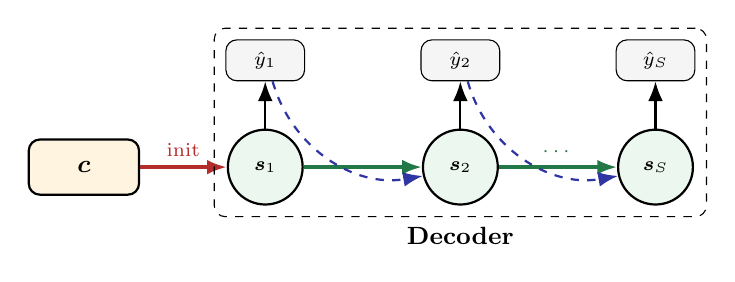
\begin{tikzpicture}[
    cell/.style={draw, circle, fill=SoftGreen!70, minimum size=0.95cm, font=\scriptsize, thick},
    io/.style={draw, rounded corners, fill=SoftGray, minimum width=1.0cm,
               minimum height=0.52cm, font=\scriptsize},
    ctx/.style={draw, rounded corners, fill=SoftOrange, minimum width=1.4cm,
                minimum height=0.7cm, font=\small, thick},
    arr/.style={-{Latex[length=2.5mm]}, thick},
    node distance=0.5cm and 1.5cm
]
\node[ctx] (c) {$\bm{c}$};
\node[cell, right=1.1cm of c] (d1) {$\bm{s}_1$};
\node[cell, right=of d1] (d2) {$\bm{s}_2$};
\node[cell, right=of d2] (dS) {$\bm{s}_S$};
\node[io, above=0.6cm of d1] (y1) {$\hat{y}_1$};
\node[io, above=0.6cm of d2] (y2) {$\hat{y}_2$};
\node[io, above=0.6cm of dS] (yS) {$\hat{y}_S$};

\draw[arr, DeepRed, very thick] (c) -- node[above,font=\scriptsize]{init} (d1);
\draw[arr, Forest, very thick] (d1) -- (d2);
\draw[arr, Forest, very thick] (d2) -- node[above,font=\scriptsize]{$\cdots$} (dS);
\draw[arr] (d1) -- (y1);
\draw[arr] (d2) -- (y2);
\draw[arr] (dS) -- (yS);
\draw[arr, dashed, CourseBlue]
    (y1) to[bend right=42] node[below,font=\scriptsize]{} (d2);
\draw[arr, dashed, CourseBlue]
    (y2) to[bend right=42] (dS);

\node[draw, dashed, rounded corners, fit=(d1)(d2)(dS)(y1)(yS),
      inner sep=4pt, label=below:{\small\textbf{Decoder}}] {};
\end{tikzpicture}
\end{center}

\begin{alertblock}{End-to-end training}
The encoder and decoder are trained jointly to maximize
$\sum_t \log P(y_t \mid y_{<t},\, \bm{x}_{1:T})$.
The gradient flows all the way from the decoder output through the context vector
back into the encoder weights.
\end{alertblock}
\end{frame}
%
%..................................................................
%
\begin{frame}{The Decoder Is a Conditional Autoregressive Model}
\small
Once the context vector $c$ is available, the decoder generates the target sequence from left to right.
At step $s$, it predicts the next token using:
\[
  \hat{p}(y_s \mid y_{<s}, c),
\]
where:
\begin{itemize}
  \item $y_s$ is the target token to be generated at position $s$;
  \item $y_{<s} = (y_1,\ldots,y_{s-1})$ denotes the previously generated target tokens;
  \item $c$ is the context vector produced by the encoder.
\end{itemize}

\vspace{0.15cm}
Therefore, the decoder is \textbf{autoregressive} because each prediction depends on previous target tokens,
and it is \textbf{conditional} because all predictions are conditioned on the source through $c$.

\begin{alertblock}{Compact description}
The encoder-decoder model is a conditional language model:
\[
  \text{language model over } y_{1:S} \quad \text{conditioned on } x_{1:T}.
\]
\end{alertblock}
\end{frame}
%
%..................................................................
%
\begin{frame}{Conditional Probability Factorization}
\small
The goal is to model the probability of the whole target sequence given the whole source sequence:
\[
  p(y_{1:S} \mid x_{1:T}).
\]
Since the encoder summarizes $x_{1:T}$ into $c$, the model approximates this as
\[
  p(y_{1:S} \mid x_{1:T}) \approx p(y_{1:S} \mid c).
\]

\vspace{0.2cm}
Using the chain rule of probability:
\[
  p(y_{1:S} \mid c)
  = \prod_{s=1}^{S} p(y_s \mid y_1,\ldots,y_{s-1}, c)
  = \prod_{s=1}^{S} p(y_s \mid y_{<s}, c).
\]

\begin{block}{Why this matters}
The decoder does not produce the whole target sentence in a single step. It produces a sequence of conditional next-token distributions.
\end{block}
\end{frame}
%
%..................................................................
%
\begin{frame}{Decoder State Update}
\small
A recurrent decoder maintains its own hidden state $s_s$ while generating the target sentence.
A common formulation is
\[
  s_0 = \phi(c),
\]
\[
  s_s = f_{\mathrm{dec}}(s_{s-1}, E_y(y_{s-1}), c),
  \qquad s=1,\ldots,S,
\]
\[
  \hat{p}(y_s \mid y_{<s},c) = \mathrm{softmax}(W_o s_s + b_o).
\]

\vspace{0.15cm}
Where:
\begin{itemize}
  \item $s_s \in \mathbb{R}^{m}$ is the decoder hidden state at output step $s$;
  \item $E_y(y_{s-1})$ is the embedding of the previous target token;
  \item $\phi$ maps the context vector into the initial decoder state;
  \item $W_o$ and $b_o$ map the decoder state to vocabulary logits.
\end{itemize}

\begin{alertblock}{Two memories interact}
The decoder state remembers what has already been generated; the context vector remembers what was read from the source.
\end{alertblock}
\end{frame}
%
%..................................................................
%
\begin{frame}{Training: Teacher Forcing}
\small
During training, the decoder usually receives the \textbf{true previous target token}, not its own previous prediction.
This is called \textbf{teacher forcing}.

\vspace{0.25cm}
For a training pair $(x_{1:T}, y_{1:S})$, the objective is to maximize
\[
  \sum_{s=1}^{S} \log p(y_s \mid y_{<s}, c),
  \qquad c = \mathrm{Encoder}(x_{1:T}).
\]
Equivalently, we minimize the negative log-likelihood:
\[
  \mathcal{L}
  = -\sum_{s=1}^{S} \log p(y_s \mid y_{<s}, c).
\]

\begin{block}{Why teacher forcing is useful}
At each output step, the model learns the correct next-token distribution under the correct previous context. This stabilizes training and makes the learning signal clearer.
\end{block}
\end{frame}
%
%..................................................................
%
\begin{frame}{Inference: Autoregressive Generation}
\small
At inference time, the true target sentence is unknown. Therefore the decoder must feed back its own predictions.

\vspace{0.25cm}
The generation loop is:
\begin{enumerate}
  \item Encode the source sequence and compute $c$.
  \item Start the decoder with a special token, usually $\langle \mathrm{start} \rangle$.
  \item Predict a probability distribution over the target vocabulary.
  \item Select the next token, for example by greedy decoding or beam search.
  \item Feed the selected token back into the decoder.
  \item Stop when $\langle \mathrm{end} \rangle$ is generated or a maximum length is reached.
\end{enumerate}

\begin{alertblock}{Important difference}
Training uses the correct previous token; inference uses the model's own previous prediction. This mismatch is one reason sequence generation can accumulate errors.
\end{alertblock}
\end{frame}
%
%..................................................................
%
\begin{frame}{The Fixed-Vector Bottleneck}
The encoder-decoder architecture is elegant but carries a fundamental structural limitation.

\vspace{0.15cm}
\begin{alertblock}{The bottleneck}
All information about the input sequence must pass through a \textbf{single fixed-size vector}
$\bm{c} \in \R^n$, regardless of how long or complex the input is.
For long documents, sentences with deep syntactic embedding, or passages requiring
multiple facts to be retained simultaneously, compressing everything into $\bm{c}$ is unreliable.
\end{alertblock}
\end{frame}
%
%..................................................................
%
\begin{frame}{The Fixed-Vector Bottleneck}
\vspace{0.15cm}
\begin{columns}[T]
\begin{column}{0.48\textwidth}
\begin{block}{Empirical evidence}
Translation quality degrades measurably for inputs beyond 20--30 tokens
(Bahdanau et al.\ 2015; Cho et al.\ 2014).
Early tokens are almost forgotten by the time the decoder starts generating.
\end{block}
\end{column}
\begin{column}{0.48\textwidth}
\begin{block}{The natural solution}
Instead of restricting the decoder to $\bm{c} = \bm{h}_T^{(e)}$, allow it to
\textbf{consult all encoder states} $\bm{h}_1^{(e)}, \ldots, \bm{h}_T^{(e)}$
at each decoding step, weighted by their relevance.
This is a step forward to\textbf{attention}.
\end{block}
\end{column}
\end{columns}
\end{frame}
%
%..................................................................
%
\begin{frame}{Why This Leads Naturally to Attention}
\small
The encoder-decoder model introduces the structure later used by attention-based models:
\begin{itemize}
  \item the \textbf{encoder} builds representations of the source sequence;
  \item the \textbf{decoder} generates the target sequence autoregressively;
  \item the target distribution is \textbf{conditioned} on source information.
\end{itemize}

\vspace{0.15cm}
In the basic model, all source information reaches the decoder only through
\[
  c = h^{(e)}_T.
\]

\begin{alertblock}{Bridge to attention}
Attention removes this rigid bottleneck. Instead of conditioning only on one vector $c$, the decoder dynamically consults all encoder states
\[
  h^{(e)}_1, h^{(e)}_2, \ldots, h^{(e)}_T.
\]
The decoder remains autoregressive, but its source conditioning becomes dynamic rather than fixed.
\end{alertblock}
\end{frame}%__________________________________________________________________________
%
\section{Conclusion and Bridge to Lesson 4}
%__________________________________________________________________________
%
\begin{frame}{What We Have Built in This Lesson}
\begin{itemize}
    \item We identified why sequential structure demands architectures with \textbf{state}:
          order fundamentally changes meaning in language.
    \item We wrote the forward-pass equations of an RNN and understood
          \textbf{parameter sharing} as the mechanism enabling variable-length processing.
    \item We derived the \textbf{vanishing gradient} from the spectral norm of a product of Jacobians
          and saw why plain RNNs have short effective memory.
    \item We saw how \textbf{gating} (GRU and LSTM) creates near-identity gradient highways,
          allowing long-range learning without exploding or vanishing.
    \item We built the \textbf{encoder-decoder architecture} for sequence-to-sequence tasks
          and identified the fixed-vector bottleneck as its principal limitation.
    \item We previewed \textbf{attention} as the mechanism that dissolves the bottleneck
          by letting the decoder consult all encoder states dynamically.
\end{itemize}

%\vspace{0.15cm}
%\begin{block}{Compact summary}
%Lesson 2a: how does a model learn a representation of a word?
%Lesson 2b: how does a model read and process a sequence of such representations?
%Lesson 3: what if we remove recurrence entirely and let tokens attend to each other directly?
%\end{block}
\end{frame}
%
%..................................................................
%
\begin{frame}{Main Takeaways}
\begin{enumerate}
    \item Sequence modeling requires architectures with \textbf{persistent state}:
          a running summary of the input that is updated at every step.
    \item BPTT reveals that training a plain RNN requires propagating gradients
          through a product of Jacobians that \textbf{vanishes exponentially} with sequence length.
    \item Gating replaces matrix multiplications on the recurrent path with
          \textbf{element-wise gated interpolation}, keeping gradients alive across long distances.
    \item GRU (2 gates) and LSTM (3 gates $+$ cell state) solve the same problem
          with different structural choices; LSTM separates memory storage from output explicitly.
    \item The encoder-decoder architecture decouples reading and generation
          but creates a \textbf{fixed-vector bottleneck} that degrades on long inputs.
    \item \textbf{Attention} replaces the fixed bottleneck with a dynamic weighted combination
          of all encoder states --- and this is the architectural seed of the transformer.
\end{enumerate}
\end{frame}
%__________________________________________________________________________
%
\section{Appendix A: BPTT Details}
%__________________________________________________________________________
%
\begin{frame}{Why We Need This Appendix}
\small
Slide 28 writes the BPTT gradient in compact matrix form. The key object is the local Jacobian
\[
\frac{\partial h_j}{\partial h_{j-1}}
\]
and, in particular, the diagonal matrix
\[
\diag\!\left(\tanh'(z_j)\right).
\]

\vspace{0.3cm}
\begin{block}{Goal of these slides}
We expand the chain rule step by step and show exactly why the derivative of the element-wise nonlinearity becomes a diagonal matrix.
\end{block}

\vspace{0.2cm}
We use column vectors. When gradients are propagated backward, the transpose of the local Jacobian appears.
\end{frame}
%
%..................................................................
%
\begin{frame}{Forward Equations and Notation}
\small
For a plain RNN, the hidden state is updated as
$$
z_t = W_h h_{t-1} + W_x x_t + b_h,
\qquad
h_t = \tanh(z_t).
$$

Where:
\begin{itemize}
    \item $x_t \in \R^d$ is the input vector at time $t$;
    \item $h_t \in \R^n$ is the hidden state at time $t$;
    \item $W_h \in \R^{n \times n}$ is the recurrent weight matrix;
    \item $W_x \in \R^{n \times d}$ maps the input into the hidden state;
    \item $b_h \in \R^n$ is the bias vector;
    \item $z_t \in \R^n$ is the pre-activation vector.
\end{itemize}

\vspace{0.15cm}
The total loss for a sequence-labeling task is usually written as
$$
L = \sum_{t=1}^{T} L_t.
$$
\end{frame}
%
%..................................................................
%
\begin{frame}{The Element-Wise Structure of the RNN Update}
\small
The $i$-th component of the pre-activation is
\[
z_{t,i} = \sum_{\ell=1}^{n} W_{h,i\ell} h_{t-1,\ell}
          + \sum_{m=1}^{d} W_{x,im} x_{t,m}
          + b_{h,i}.
\]

The $i$-th component of the hidden state is then
\[
h_{t,i} = \tanh(z_{t,i}).
\]

\vspace{0.2cm}
\begin{block}{Crucial observation}
The activation function is applied \textbf{component by component}. Therefore $h_{t,i}$ depends directly on $z_{t,i}$, but not directly on $z_{t,r}$ for $r \neq i$.
\end{block}

This component-wise dependence is what produces a diagonal Jacobian.
\end{frame}
%
%..................................................................
%
\begin{frame}{Deriving the Diagonal Term}
\small
Consider the Jacobian of $h_t$ with respect to $z_t$:
\[
\frac{\partial h_t}{\partial z_t}
= \left[\frac{\partial h_{t,i}}{\partial z_{t,r}}\right]_{i,r=1}^{n}.
\]

Since
\[
h_{t,i} = \tanh(z_{t,i}),
\]
we have
\[
\frac{\partial h_{t,i}}{\partial z_{t,r}}
= 
\begin{cases}
\tanh'(z_{t,i}), & \text{if } i=r,\\[4pt]
0, & \text{if } i \neq r.
\end{cases}
\]

Therefore,
\[
\frac{\partial h_t}{\partial z_t}
= \diag\!\left(\tanh'(z_t)\right).
\]

\begin{alertblock}{Interpretation}
The diagonal matrix appears because the nonlinearity mixes no coordinates: each output component only differentiates with respect to its own input component.
\end{alertblock}
\end{frame}
%
%..................................................................
%
\begin{frame}{The Local Jacobian Through One Recurrent Step}
\small
We now compute
\[
\frac{\partial h_t}{\partial h_{t-1}}.
\]

By the chain rule:
\[
\frac{\partial h_t}{\partial h_{t-1}}
= \frac{\partial h_t}{\partial z_t}
  \frac{\partial z_t}{\partial h_{t-1}}.
\]

From the previous slide,
\[
\frac{\partial h_t}{\partial z_t}
= \diag\!\left(\tanh'(z_t)\right).
\]

Since $z_t = W_h h_{t-1} + W_x x_t + b_h$, we get
\[
\frac{\partial z_t}{\partial h_{t-1}} = W_h.
\]

Hence the forward local Jacobian is
\[
\boxed{
\frac{\partial h_t}{\partial h_{t-1}}
= \diag\!\left(\tanh'(z_t)\right) W_h
}
\]
\end{frame}
%
%..................................................................
%
\begin{frame}{Backward Propagation Uses the Transposed Jacobian}
\small
Let
\[
\delta_t^{(h)} = \frac{\partial L}{\partial h_t}
\]
be the gradient arriving at time $t$. To move it one step backward, we use the transpose of the local Jacobian:
\[
\delta_{t-1}^{(h)}
= \left(\frac{\partial h_t}{\partial h_{t-1}}\right)^{\top}
\delta_t^{(h)}.
\]

Using the result from the previous slide:
\[
\delta_{t-1}^{(h)}
= \left[\diag\!\left(\tanh'(z_t)\right) W_h\right]^{\top}
\delta_t^{(h)}.
\]

Since a diagonal matrix is symmetric,
\[
\diag\!\left(\tanh'(z_t)\right)^{\top}
= \diag\!\left(\tanh'(z_t)\right),
\]
we obtain
\[
\boxed{
\delta_{t-1}^{(h)}
= W_h^{\top}\diag\!\left(\tanh'(z_t)\right)\delta_t^{(h)}.
}
\]

This is the factor appearing in the BPTT formula.
\end{frame}
%
%..................................................................
%
\begin{frame}{From One Step to Many Steps: The Product of Jacobians}
\small
For a loss term $L_t$, the gradient must travel from $h_t$ back to an earlier hidden state $h_k$, with $k<t$.

Applying the previous recurrence repeatedly gives
\[
\delta_k^{(h,t)}
=
\left(
\prod_{j=k+1}^{t}
W_h^{\top}\diag\!\left(\tanh'(z_j)\right)
\right)
\delta_t^{(h)}.
\]

Equivalently, in compact chain-rule notation,
\[
\frac{\partial L_t}{\partial h_k}
=
\frac{\partial L_t}{\partial h_t}
\left(
\prod_{j=k+1}^{t}
\frac{\partial h_j}{\partial h_{j-1}}
\right),
\]
with the appropriate transpose depending on whether gradients are represented as row or column vectors.

\begin{block}{Meaning}
BPTT is ordinary backpropagation applied to the RNN unrolled over time. The only new feature is that the same matrix $W_h$ appears at every step.
\end{block}
\end{frame}
%
%..................................................................
%
\begin{frame}{Gradient with Respect to the Recurrent Matrix $W_h$}
\small
The contribution of $L_t$ to the gradient of $W_h$ comes from every previous time step $k \leq t$:
\[
\frac{\partial L_t}{\partial W_h}
= \sum_{k=1}^{t}
\frac{\partial L_t}{\partial z_k}
\frac{\partial z_k}{\partial W_h}.
\]

Define
\[
\delta_k^{(z,t)} = \frac{\partial L_t}{\partial z_k}.
\]

Since
\[
z_k = W_h h_{k-1} + W_x x_k + b_h,
\]
the matrix derivative has the outer-product form
\[
\boxed{
\frac{\partial L_t}{\partial W_h}
= \sum_{k=1}^{t}
\delta_k^{(z,t)} h_{k-1}^{\top}.
}
\]

The compact formula on slide 28 expresses the same idea: each term in the sum contains a gradient transported backward through a product of recurrent Jacobians.
\end{frame}
%
%..................................................................
%
\begin{frame}{Why This Leads to Vanishing Gradients}
\small
Each backward step contains the factor
\[
W_h^{\top}\diag\!\left(\tanh'(z_j)\right).
\]

The derivative of the hyperbolic tangent is
\[
\tanh'(u) = 1 - \tanh^2(u).
\]

Therefore,
\[
0 < \tanh'(u) \leq 1.
\]

\vspace{0.15cm}
If $z_{j,i}$ is in the saturated region of $\tanh$, then
\[
\tanh'(z_{j,i}) \approx 0.
\]

\begin{alertblock}{Consequence}
The diagonal term can strongly shrink some coordinates of the gradient. When this shrinkage is multiplied across many time steps, the gradient can decay exponentially.
\end{alertblock}

This is the mathematical core of the vanishing-gradient problem for plain RNNs.
\end{frame}
%
%..................................................................
%
\begin{frame}{Column vs. Row Convention: Why the Order May Look Different}
\small
With column gradients, the one-step backward recursion is
\[
\delta_{t-1}^{(h)}
= W_h^{\top}\diag\!\left(\tanh'(z_t)\right)\delta_t^{(h)}.
\]

With row gradients, the same relationship is often written as
\[
\frac{\partial L}{\partial h_{t-1}}
= \frac{\partial L}{\partial h_t}
\diag\!\left(\tanh'(z_t)\right) W_h.
\]

\vspace{0.2cm}
\begin{block}{Important point}
The mathematical content is the same. The difference is only whether gradients are written as column vectors or row vectors. In both cases, the diagonal term comes from differentiating the element-wise $\tanh$ activation.
\end{block}

\vspace{0.1cm}
The essential BPTT structure remains a product of local Jacobians across time.
\end{frame}
%
%..................................................................
%
\begin{frame}{Takeaway}
\small
The BPTT formula on slide 28 is just repeated application of the chain rule through the unrolled RNN.

\vspace{0.25cm}
The diagonal matrix
\[
\diag\!\left(\tanh'(z_j)\right)
\]
appears because $\tanh$ is applied independently to each coordinate of $z_j$.

\vspace{0.25cm}
The recurrent matrix $W_h$ appears because each pre-activation $z_j$ depends linearly on the previous hidden state $h_{j-1}$:
\[
z_j = W_h h_{j-1} + W_x x_j + b_h.
\]

\vspace{0.25cm}
Therefore, every backward step contains a Jacobian factor of the form
\[
W_h^{\top}\diag\!\left(\tanh'(z_j)\right),
\]
and multiplying many such factors explains why gradients in plain RNNs may vanish or explode.
\end{frame}
%__________________________________________________________________________
%
\section{Appendix B: Gate Equation}
%__________________________________________________________________________
%
\begin{frame}{Why This Notation Appears}

A gate in a recurrent network usually depends on two pieces of information:

\vspace{0.15cm}

\begin{itemize}
  \item $h_{t-1}$: the previous hidden state, summarizing the past;
  \item $x_t$: the current input vector, representing the token observed now.
\end{itemize}

\vspace{0.25cm}

A typical gate equation is

\[
  z_t = \sigma\left(W_z [h_{t-1}, x_t] + b_z\right).
\]

The expression $[h_{t-1}, x_t]$  means: \textbf{concatenate the two vectors into one longer vector}.

\end{frame}
%
%..................................................................
%
\begin{frame}{The Dimensions of the Two Vectors}

Let

\[
  h_{t-1} \in \mathbb{R}^{n}
\]

be the previous hidden state, where $n$ is the number of hidden units.

\vspace{0.2cm}

Let

\[
  x_t \in \mathbb{R}^{d}
\]

be the current input vector, where $d$ is the input embedding dimension.

\vspace{0.25cm}

Then the concatenated vector is

\[
  [h_{t-1}, x_t]
  =
  \begin{bmatrix}
    h_{t-1} \\
    x_t
  \end{bmatrix}
  \in \mathbb{R}^{n+d}.
\]

\end{frame}
%
%..................................................................
%
\begin{frame}{From Two Vectors to One Matrix-Vector Product}

After concatenation, the model is no longer multiplying a matrix by two separate vectors.

\vspace{0.2cm}

It is multiplying a matrix by one vector of length $n+d$:

\[
  W_z [h_{t-1},x_t].
\]

If the gate has dimension $n$, then

\[
  W_z \in \mathbb{R}^{n \times (n+d)},
  \qquad
  b_z \in \mathbb{R}^{n}.
\]

Therefore

\[
  W_z [h_{t-1},x_t] + b_z \in \mathbb{R}^{n}.
\]

The output has the same dimension as the hidden state, because the gate controls the hidden state component by component.

\end{frame}
%
%..................................................................
%
\begin{frame}{A Concrete Shape Example}

Suppose

\[
  h_{t-1}
  =
  \begin{bmatrix}
  h_1 \\
  h_2 \\
  h_3
  \end{bmatrix}
  \in \mathbb{R}^{3},
  \qquad
  x_t
  =
  \begin{bmatrix}
  x_1 \\
  x_2
  \end{bmatrix}
  \in \mathbb{R}^{2}.
\]

Then the concatenated vector is

\[
  [h_{t-1}, x_t]
  =
  \begin{bmatrix}
  h_1 \\
  h_2 \\
  h_3 \\
  x_1 \\
  x_2
  \end{bmatrix}
  \in \mathbb{R}^{5}.
\]

If $z_t \in \mathbb{R}^{3}$, then

\[
  W_z \in \mathbb{R}^{3\times 5},
  \qquad
  b_z \in \mathbb{R}^{3}.
\]

\end{frame}
%
%..................................................................
%
\begin{frame}{Equivalent Block-Matrix Interpretation}
\small

The compact notation

\[
  W_z [h_{t-1}, x_t]
\]

can be rewritten by splitting $W_z$ into two blocks:

\[
  W_z = \begin{bmatrix} W_{zh} & W_{zx} \end{bmatrix},
\]

where

\[
  W_{zh} \in \mathbb{R}^{n \times n},
  \qquad
  W_{zx} \in \mathbb{R}^{n \times d}.
\]

Then

\[
  W_z
  \begin{bmatrix}
  h_{t-1} \\
  x_t
  \end{bmatrix}
  =
  W_{zh} h_{t-1} + W_{zx} x_t.
\]

The gate combines transformed information from the past state and the current input.

\end{frame}
%
%..................................................................
%
\begin{frame}{From Linear Score to Gate Value}

First compute a pre-activation vector:

\[
  u_t = W_z [h_{t-1}, x_t] + b_z.
\]

Then apply the sigmoid element by element:

\[
  z_t = \sigma(u_t),
  \qquad
  \sigma(u) = \frac{1}{1+e^{-u}}.
\]

Since the sigmoid maps real numbers into $(0,1)$,

\[
  z_t \in (0,1)^n.
\]

Each component $z_{t,i}$ is an interpolation coefficient.  
It tells the recurrent cell how much to update or preserve component $i$ of the state.

\end{frame}
%
%..................................................................
%
\begin{frame}{Implementation View}

In code, the mathematical concatenation

\[
  [h_{t-1},x_t]
\]

corresponds to concatenating tensors along the feature dimension.

\vspace{0.25cm}

For a single example:

\[
  h_{t-1}: (n),
  \qquad
  x_t: (d),
  \qquad
  [h_{t-1},x_t]: (n+d).
\]

For a batch of $B$ examples:

\[
  h_{t-1}: (B,n),
  \qquad
  x_t: (B,d),
  \qquad
  [h_{t-1},x_t]: (B,n+d).
\]

The brackets $[\cdot,\cdot]$ are mathematical notation for concatenation. They should not be confused with an ordinary list containing two separate objects.

\end{frame}
%
%===================================================================================================
%
\end{document}
%
%===================================================================================================
%
